\documentclass[12pt,oneside]{book}

%% --- Packages ---
\usepackage[utf8]{inputenc}
\usepackage[T1]{fontenc}
\usepackage[spanish]{babel}
\usepackage{geometry}
\geometry{left=2.5cm,right=2.5cm,top=3cm,bottom=3cm,headheight=15pt}
\usepackage{graphicx}
\usepackage{hyperref}
\usepackage{listings}
\usepackage{xcolor}
\usepackage{float}
\usepackage{caption}
\usepackage{subcaption}
\usepackage{booktabs}
\usepackage{longtable}
\usepackage{array}
\usepackage{enumitem}
\usepackage{fancyhdr}
\usepackage{titlesec}
\usepackage{setspace}
\usepackage{verbatim}
%% --- Colors for listings ---
\definecolor{codegreen}{rgb}{0,0.6,0}
\definecolor{codegray}{rgb}{0.5,0.5,0.5}
\definecolor{codepurple}{rgb}{0.58,0,0.82}
\definecolor{backcolour}{rgb}{0.95,0.95,0.92}

\lstdefinestyle{mystyle}{
    backgroundcolor=\color{backcolour},
    commentstyle=\color{codegreen},
    keywordstyle=\color{magenta},
    numberstyle=\tiny\color{codegray},
    stringstyle=\color{codepurple},
    basicstyle=\ttfamily\footnotesize,
    breakatwhitespace=false,
    breaklines=true,
    captionpos=b,
    keepspaces=true,
    numbers=left,
    numbersep=5pt,
    showspaces=false,
    showstringspaces=false,
    showtabs=false,
    tabsize=2
}
\lstset{style=mystyle}

\lstdefinelanguage{JavaScript}{
    keywords={async, await, break, case, catch, class, const, continue, debugger, default, delete, do, else, export, extends, false, finally, for, function, if, import, in, instanceof, let, new, null, of, return, super, switch, this, throw, true, try, typeof, var, void, while, with, yield},
    sensitive=true,
    comment=[l]{//},
    morecomment=[s]{/*}{*/},
    morestring=[b]',
    morestring=[b]"
}

\lstdefinelanguage{Java}{
    keywords={abstract, assert, boolean, break, byte, case, catch, class, const, continue, default, do, double, else, enum, extends, false, final, finally, float, for, goto, if, implements, import, instanceof, int, interface, long, native, new, null, package, private, protected, public, return, short, static, strictfp, super, switch, synchronized, this, throw, throws, transient, true, try, void, volatile, while},
    sensitive=true,
    comment=[l]{//},
    morecomment=[s]{/*}{*/},
    morestring=[b]',
    morestring=[b]"
}

%% --- Header / Footer ---
\pagestyle{fancy}
\fancyhf{}
\fancyhead[L]{\leftmark}
\fancyhead[R]{PetClinic}
\fancyfoot[C]{\thepage}

%% --- Title formatting ---
\titleformat{\chapter}[display]
  {\normalfont\huge\bfseries}{\chaptertitlename\ \thechapter}{20pt}{\Huge}
\titleformat{\section}
  {\normalfont\Large\bfseries}{\thesection}{1em}{}
\titleformat{\subsection}
  {\normalfont\large\bfseries}{\thesubsection}{1em}{}

%% --- Metadata ---
\title{
    \vspace*{3cm}
    {\Huge \textbf{PetClinic}}\\[0.5cm]
    {\Large Sistema de Gesti\'on de Cl\'inica Veterinaria}\\[0.5cm]
    {\large Documentaci\'on T\'ecnica del Proyecto}
}
\author{Departamento de Desarrollo}
\date{\today}

\begin{document}

\maketitle
\thispagestyle{empty}
\newpage

\tableofcontents
\newpage

\listoffigures
\newpage

\lstlistoflistings
\newpage

%% --- Include chapters ---
\chapter{Introducci\'on}

\section{Descripci\'on del Proyecto}

PetClinic es un sistema de gesti\'on para cl\'inicas veterinarias desarrollado como aplicaci\'on web moderna. El sistema permite administrar todos los aspectos operativos de una cl\'inica veterinaria: gesti\'on de clientes, pacientes (mascotas), citas, facturaci\'on, inventario de medicamentos, historial m\'edico, hospitalizaci\'on, planes de tratamiento, consentimientos informados, odontograma canino, y m\'as.

El proyecto est\'a construido con una arquitectura de capas utilizando Java 21 y Spring Boot 3.2.3 en el backend, con una base de datos PostgreSQL, y un frontend SPA (\textit{Single-Page Application}) construido con Bootstrap 5, FullCalendar 6 y Chart.js.

\subsection{Objetivos del Sistema}

\begin{itemize}
    \item Digitalizar y centralizar la informaci\'on de pacientes y clientes.
    \item Facilitar la gesti\'on de citas con un calendario interactivo.
    \item Automatizar la facturaci\'on con generaci\'on de PDF y control de inventario.
    \item Proveer un portal de cliente para consulta de citas y facturas.
    \item Implementar alertas autom\'aticas de vacunaci\'on v\'ia correo electr\'onico.
    \item Gestionar hospitalizaciones, planes de tratamiento y consentimientos.
    \item Incluir un odontograma canino interactivo para diagn\'ostico dental.
    \item Integrar pagos en l\'inea mediante Stripe.
\end{itemize}

\subsection{P\'ublico Objetivo}

El sistema est\'a dise\~nado para:

\begin{itemize}
    \item \textbf{Administradores:} Control total del sistema, gesti\'on de usuarios y auditor\'ia.
    \item \textbf{Veterinarios:} Gesti\'on cl\'inica completa (citas, historial, facturaci\'on).
    \item \textbf{Recepcionistas:} Lectura de datos y creaci\'on de clientes/citas.
    \item \textbf{Clientes:} Portal propio para consultar citas, facturas e historial de mascotas.
\end{itemize}

\section{Tecnolog\'ias Utilizadas}

\subsection{Lenguaje y Framework}

\begin{itemize}
    \item \textbf{Java 21:} \'Ultima versi\'on LTS con caracter\'isticas modernas como \textit{Pattern Matching}, \textit{Records}, y \textit{Sealed Classes}.
    \item \textbf{Spring Boot 3.2.3:} Framework de aplicaciones que simplifica la configuraci\'on y el despliegue.
    \item \textbf{Spring Data JPA / Hibernate:} ORM para la capa de persistencia.
    \item \textbf{Spring Security:} Framework de autenticaci\'on y autorizaci\'on.
    \item \textbf{Spring WebSocket:} Comunicaci\'on en tiempo real para notificaciones de citas.
    \item \textbf{Spring Mail:} Env\'io de correos electr\'onicos (alertas de vacunas, recordatorios).
    \item \textbf{Spring AOP:} Programaci\'on orientada a aspectos.
\end{itemize}

\subsection{Base de Datos}

\begin{itemize}
    \item \textbf{PostgreSQL 14+:} Base de datos relacional en producci\'on.
    \item \textbf{H2:} Base de datos en memoria para pruebas.
\end{itemize}

\subsection{Seguridad}

\begin{itemize}
    \item \textbf{JJWT 0.12.3:} Biblioteca para generaci\'on y validaci\'on de tokens JWT.
    \item \textbf{BCrypt:} Algoritmo de hashing para contrase\~nas.
\end{itemize}

\subsection{Frontend}

\begin{itemize}
    \item \textbf{Bootstrap 5.3:} Framework CSS para dise\~no responsive.
    \item \textbf{Bootstrap Icons:} Conjunto de iconos vectoriales.
    \item \textbf{FullCalendar 6.1:} Calendario interactivo para gesti\'on de citas.
    \item \textbf{Chart.js 4.4:} Biblioteca de gr\'aficos para reportes.
    \item \textbf{Vanilla JS:} JavaScript nativo sin frameworks adicionales, con patr\'on de m\'odulos por secci\'on.
\end{itemize}

\subsection{Otras Tecnolog\'ias}

\begin{itemize}
    \item \textbf{iText 7 Core 8.0.3:} Generaci\'on de PDFs (facturas, consentimientos).
    \item \textbf{Apache POI 5.2.5:} Generaci\'on de archivos Excel (reportes de ingresos).
    \item \textbf{Stripe Java 28.1.0:} Integraci\'on de pagos en l\'inea.
    \item \textbf{Maven:} Herramienta de construcci\'on y gesti\'on de dependencias.
    \item \textbf{JUnit 5:} Framework de pruebas unitarias y de integraci\'on.
\end{itemize}

\section{Convenciones del Proyecto}

\begin{itemize}
    \item \textbf{Arquitectura en capas:} Controller $\rightarrow$ Service $\rightarrow$ Repository $\rightarrow$ DB.
    \item \textbf{DTO Pattern:} Separaci\'on de entidades JPA de los objetos de transferencia de datos.
    \item \textbf{Inyecci\'on de dependencias:} Constructor injection en todas las clases.
    \item \textbf{Global Exception Handler:} Manejo centralizado de excepciones con \texttt{@RestControllerAdvice}.
    \item \textbf{Auditor\'ia:} Registro de acciones CRUD con detalles de usuario y direcci\'on IP.
    \item \textbf{WebSocket:} Notificaciones en tiempo real para cambios en citas.
\end{itemize}

\section{Requisitos del Sistema}

\begin{itemize}
    \item Java 21 o superior.
    \item PostgreSQL 14 o superior.
    \item Maven 3.8+.
    \item Navegador web moderno (Chrome, Firefox, Edge).
    \item (Opcional) Cuenta de Stripe para pagos en l\'inea.
    \item (Opcional) Cuenta SMTP para env\'io de correos.
\end{itemize}

\chapter{Arquitectura del Sistema}

\section{Visi\'on General}

PetClinic sigue una arquitectura en capas (\textit{Layered Architecture}) con una SPA (\textit{Single Page Application}) en el frontend que se comunica con el backend mediante una API REST protegida con JWT. El backend sigue el patr\'on Controller $\rightarrow$ Service $\rightarrow$ Repository $\rightarrow$ DB, con una separaci\'on estricta de responsabilidades.

\begin{figure}[H]
    \centering
    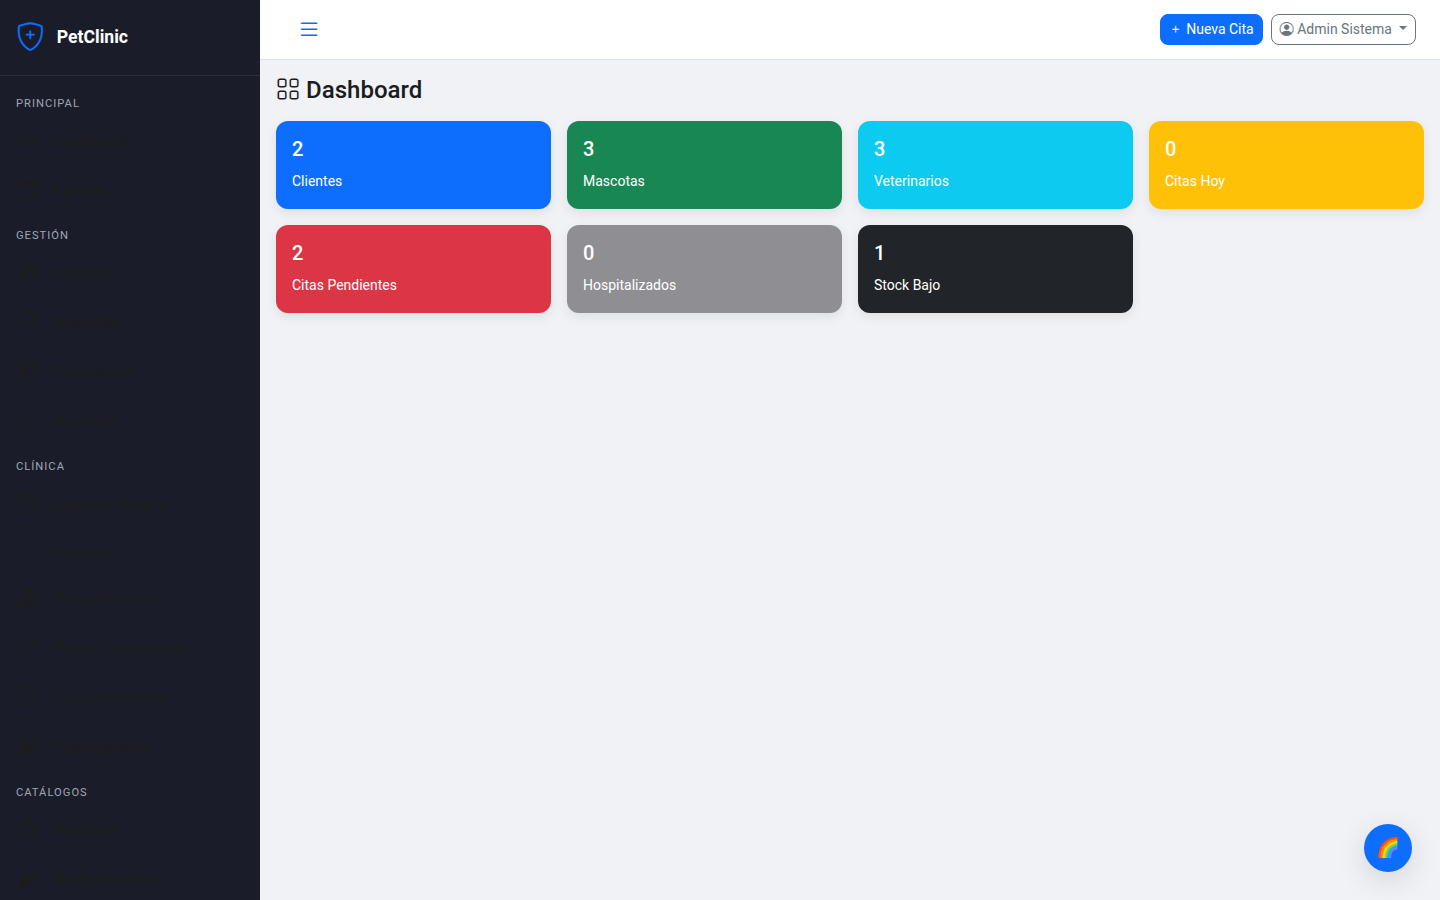
\includegraphics[width=0.9\textwidth]{images/02-dashboard}
    \caption{Pantalla principal del Dashboard de PetClinic}
    \label{fig:dashboard}
\end{figure}

\subsection{Diagrama de Capas}

\begin{verbatim}
+------------------------------------------------------------------+
|  Cliente (SPA: HTML + CSS + Vanilla JS)                           |
|  - Bootstrap 5.3 (responsive)  - FullCalendar 6.1 (agenda)       |
|  - Chart.js 4.4 (graficos)     - Bootstrap Icons                  |
+------------------------------------------------------------------+
        |  HTTP/JSON + JWT (Bearer token en header Authorization)
        v
+------------------------------------------------------------------+
|  Controller Layer (REST API)    20 controladores                  |
|  - DTO validation con Jakarta Validation                         |
|  - @RestController + @RequestMapping                             |
+------------------------------------------------------------------+
        |
        v
+------------------------------------------------------------------+
|  Service Layer (Logica de negocio)  22 servicios                  |
|  - @Transactional para operaciones atomicas                      |
|  - Inyeccion de dependencias via constructor                      |
|  - Orquestacion, calculos, reglas de negocio                      |
+------------------------------------------------------------------+
        |
        v
+------------------------------------------------------------------+
|  Repository Layer (Spring Data JPA)  19 repositorios              |
|  - JpaRepository<T, Long> con consultas derivadas                 |
|  - JPQL para consultas personalizadas                             |
|  - Paginacion y ordenamiento                                      |
+------------------------------------------------------------------+
        |
        v
+------------------------------------------------------------------+
|  Base de Datos (PostgreSQL 14+)                                   |
|  19 tablas principales + 1 tabla de auditoria                     |
+------------------------------------------------------------------+
\end{verbatim}

\section{Flujo de una Petici\'on}

Cada petici\'on HTTP atraviesa los siguientes componentes en orden:

\begin{enumerate}
    \item \textbf{JwtAuthFilter:} Extrae el token del header \texttt{Authorization: Bearer <token>}, valida la firma HMAC-SHA384, verifica expiraci\'on y extrae los claims (email, rol, userId). Si es v\'alido, establece la autenticaci\'on en el \texttt{SecurityContextHolder}.
    \item \textbf{SecurityConfig:} Verifica que el rol del usuario (ADMIN, VETERINARIO, RECEPCIONISTA, CLIENTE) tenga permiso para el endpoint solicitado mediante reglas \texttt{authorizeHttpRequests}.
    \item \textbf{Controller:} Recibe la petici\'on HTTP, valida los DTOs con \texttt{@Valid} y \texttt{jakarta.validation}, y delega la l\'ogica al servicio correspondiente.
    \item \textbf{Service:} Ejecuta la l\'ogica de negocio dentro de una transacci\'on (\texttt{@Transactional}). Realiza validaciones, c\'alculos y orquestaci\'on de operaciones.
    \item \textbf{Repository:} Interact\'ua con la base de datos mediante Spring Data JPA. Las consultas personalizadas se definen con JPQL.
    \item \textbf{GlobalExceptionHandler:} Captura cualquier excepci\'on no manejada y la formatea como una respuesta JSON est\'andar con c\'odigo HTTP apropiado.
\end{enumerate}

\section{Flujo de Notificaciones en Tiempo Real (WebSocket)}

PetClinic utiliza WebSocket con STOMP sobre SockJS para notificaciones en tiempo real de cambios en citas.

\begin{verbatim}
+--------+          +------------------+          +--------------+
| Cliente|          |  Spring Backend  |          |  Otros       |
| SPA    |          |  (CitaController)|          |  Clientes    |
+--------+          +------------------+          +--------------+
    |                     |                            |
    |  POST /api/medico/  |                            |
    |  citas (crear cita) |                            |
    |-------------------->|                            |
    |                     |                            |
    |  200 OK (cita Creada)|                           |
    |<--------------------|                            |
    |                     |                            |
    |                     |  conversionService         |
    |                     |  .broadcast("/topic/citas", |
    |                     |    citaDto)                |
    |                     |--------------------------->|
    |                     |                            |
    |  STOMP message      |                            |
    |  /topic/citas       |                            |
    |<--------------------|                            |
    |                     |                            |
\end{verbatim}

La configuraci\'on WebSocket se implementa de la siguiente manera:

\begin{lstlisting}[language=Java, caption=Configuraci\'on WebSocket]
@Configuration
@EnableWebSocketMessageBroker
public class WebSocketConfig implements WebSocketMessageBrokerConfigurer {
    @Override
    public void configureMessageBroker(MessageBrokerRegistry config) {
        config.enableSimpleBroker("/topic");
        config.setApplicationDestinationPrefixes("/app");
    }

    @Override
    public void registerStompEndpoints(StompEndpointRegistry registry) {
        registry.addEndpoint("/ws")
                .setAllowedOriginPatterns("*")
                .withSockJS();
    }
}
\end{lstlisting}

\section{Patrones de Dise\~no}

\subsection{Patrones Implementados}

\begin{longtable}{|p{4cm}|p{10cm}|}
\hline
\textbf{Patr\'on} & \textbf{Implementaci\'on} \\
\hline
Singleton & Spring Beans (\texttt{@Service}, \texttt{@Repository}, \texttt{@Controller}) \\
\hline
Inyecci\'on de Dependencias & Constructor injection en todas las clases \\
\hline
Factory & Spring Data JPA genera repositorios autom\'aticamente \\
\hline
Chain of Responsibility & Security Filter Chain (\texttt{JwtAuthFilter} $\rightarrow$ \texttt{UsernamePasswordAuthenticationFilter}) \\
\hline
Observer / Pub-Sub & WebSocket STOMP para actualizaciones de citas en tiempo real \\
\hline
Strategy & \texttt{PasswordEncoder} (BCrypt) intercambiable \\
\hline
Template Method & JPA Lifecycle Callbacks (\texttt{@PrePersist}, \texttt{@PreUpdate}) \\
\hline
DTO Pattern & \texttt{CitaDto}, \texttt{FacturaDto}, \texttt{LoginRequest/Response} separan API de entidades \\
\hline
Global Exception Handler & \texttt{@RestControllerAdvice} con \texttt{GlobalExceptionHandler} \\
\hline
CommandLineRunner & \texttt{DataInitializer} para seed data al arrancar \\
\hline
DAO Pattern & Repositorios encapsulan operaciones de base de datos \\
\hline
Scheduling & \texttt{@Scheduled} en \texttt{VacunaScheduler} para alertas autom\'aticas \\
\hline
Facade & Servicios act\'uan como fachada ante operaciones complejas (ej: \texttt{FacturaService}) \\
\hline
\end{longtable}

\section{Diagrama de Componentes}

\subsection{Capas del Sistema}

\paragraph{Capa de Presentaci\'on (Frontend)}
SPA construida con HTML, CSS y JavaScript vanilla. Utiliza Bootstrap 5 para el dise\~no responsive, FullCalendar 6 para la agenda de citas, Chart.js 4 para gr\'aficos de reportes. Se comunica con el backend mediante peticiones HTTP REST con autenticaci\'on JWT. Las actualizaciones en tiempo real llegan v\'ia WebSocket STOMP.

\paragraph{Capa de API REST (Controller)}
20 controladores REST que exponen endpoints para cada m\'odulo del sistema. Los controladores reciben y devuelven DTOs, nunca entidades JPA directamente. Utilizan \texttt{@Valid} para validaci\'on autom\'atica de entrada y \texttt{ResponseEntity} para control de c\'odigos HTTP.

\paragraph{Capa de Negocio (Service)}
22 servicios que encapsulan toda la l\'ogica de negocio. Los servicios son transaccionales y contienen validaciones, c\'alculos y orquestaci\'on de operaciones. Ejemplos: \texttt{CitaService} valida disponibilidad, \texttt{FacturaService} maneja descuento de stock, \texttt{PdfService} genera documentos.

\paragraph{Capa de Persistencia (Repository)}
19 interfaces de repositorio que extienden \texttt{JpaRepository} con consultas personalizadas mediante JPQL y m\'etodos derivados. Cada repositorio incluye consultas espec\'ificas como b\'usqueda por texto libre, agregaciones y filtros por estado.

\paragraph{Capa de Seguridad}
4 componentes de seguridad: \texttt{JwtTokenProvider} genera y valida tokens, \texttt{JwtAuthFilter} intercepta peticiones, \texttt{SecurityConfig} configura reglas de acceso, \texttt{CustomUserDetailsService} carga usuarios de la base de datos.

\section{Esquema de Navegaci\'on}

La aplicaci\'on cuenta con dos modos de navegaci\'on:

\begin{itemize}
    \item \textbf{Modo Staff (Personal):} Barra lateral con secciones para administraci\'on cl\'inica (Dashboard, Agenda, Clientes, Mascotas, Facturaci\'on, Reportes, Historial M\'edico, Vacunas, Hospitalizaci\'on, Planes, Consentimientos, Odontograma, Servicios, Medicamentos, Admin, Auditor\'ia, Configuraci\'on).
    \item \textbf{Modo Cliente:} Barra lateral simplificada con secciones personales (Inicio, Mis Mascotas, Mis Citas, Mis Facturas, Mi Perfil).
\end{itemize}

\chapter{Modelo de Datos}

\section{Diagrama Entidad-Relaci\'on}

El sistema cuenta con 19 tablas principales m\'as 1 tabla de auditor\'ia. JPA genera autom\'aticamente el esquema con \texttt{spring.jpa.hibernate.ddl-auto=update}.

\subsection{Entidades del Sistema}

\subsubsection*{Veterinario (veterinarios)}
Almacena los usuarios del sistema: administradores, veterinarios y recepcionistas.
\begin{lstlisting}[language=Java, caption=Entidad Veterinario]
@Entity @Table(name = "veterinarios")
public class Veterinario {
    @Id @GeneratedValue(strategy = GenerationType.IDENTITY)
    private Long id;
    @NotBlank private String nombre;
    @NotBlank private String apellido;
    @NotBlank @Column(unique = true) private String email;
    @NotBlank private String passwordHash;  // BCrypt
    private String telefono;
    private String especialidad;
    private String cedulaProfesional;
    @Enumerated(EnumType.STRING) private RolUsuario rol;
    private LocalTime horarioInicio;
    private LocalTime horarioFin;
    private Integer duracionTurnoMinutos = 30;
    private Boolean activo = true;
    // Auditoria: createdAt, updatedAt
}
\end{lstlisting}

\subsubsection*{Cliente (clientes)}
Due\~nos de mascotas con opci\'on de portal web.
\begin{lstlisting}[language=Java, caption=Entidad Cliente]
@Entity @Table(name = "clientes")
public class Cliente {
    @Id @GeneratedValue(strategy = GenerationType.IDENTITY)
    private Long id;
    @NotBlank private String nombre;
    @NotBlank private String apellido;
    @Email @NotBlank private String email;
    private String telefono;
    private String direccion;
    private String portalEmail;          // Login para portal cliente
    private String portalPasswordHash;   // BCrypt
    private Boolean portalActivo = false;
    @OneToMany(mappedBy = "cliente") private List<Mascota> mascotas;
}
\end{lstlisting}

\subsubsection*{Mascota (mascotas)}
Pacientes del sistema, vinculados a un cliente due\~no.
\begin{lstlisting}[language=Java, caption=Entidad Mascota]
@Entity @Table(name = "mascotas")
public class Mascota {
    @Id @GeneratedValue(strategy = GenerationType.IDENTITY)
    private Long id;
    @NotBlank private String nombre;
    @Enumerated(EnumType.STRING) private Especie especie;
    private String raza, color;
    @Enumerated(EnumType.STRING) private GeneroMascota genero;
    private LocalDate fechaNacimiento;
    private Double peso;
    @Column(columnDefinition = "TEXT") private String alergias;
    @Column(columnDefinition = "TEXT") private String condicionesMedicas;
    @ManyToOne @JoinColumn(name = "cliente_id") private Cliente cliente;
}
\end{lstlisting}

\subsubsection*{Cita (citas)}
Agendamiento de consultas con control de disponibilidad.
\begin{lstlisting}[language=Java, caption=Entidad Cita]
@Entity @Table(name = "citas")
public class Cita {
    @Id @GeneratedValue(strategy = GenerationType.IDENTITY)
    private Long id;
    @ManyToOne private Mascota mascota;
    @ManyToOne private Veterinario veterinario;
    @ManyToOne private Cliente cliente;
    @NotNull private LocalDateTime fechaHoraInicio;
    @NotNull private LocalDateTime fechaHoraFin;
    @NotBlank private String motivo;
    @Column(columnDefinition = "TEXT") private String notas;
    @Enumerated(EnumType.STRING) private EstadoCita estado;
    private String motivoCancelacion;
}
\end{lstlisting}

\subsubsection*{Factura (facturas)}
Facturaci\'on con detalle de items y control de pagos.
\begin{lstlisting}[language=Java, caption=Entidad Factura]
@Entity @Table(name = "facturas")
public class Factura {
    @Id @GeneratedValue(strategy = GenerationType.IDENTITY)
    private Long id;
    @NotBlank @Column(unique = true) private String numeroFactura;
    @ManyToOne private Cliente cliente;
    @ManyToOne private Veterinario veterinario;
    @ManyToOne private Cita cita;  // Opcional
    private LocalDateTime fechaEmision;
    private Double subtotal = 0.0;
    private Double descuentoTotal = 0.0;
    private Double total = 0.0;
    @Enumerated(EnumType.STRING) private EstadoFactura estado;
    private Double totalPagado = 0.0;
    @OneToMany(mappedBy = "factura", cascade = CascadeType.ALL)
    private List<DetalleFactura> detalles;
    @OneToMany(mappedBy = "factura", cascade = CascadeType.ALL)
    private List<Pago> pagos;
}
\end{lstlisting}

\subsection{Enumeraciones}

\begin{longtable}{|p{4cm}|p{10cm}|}
\hline
\textbf{Enumeraci\'on} & \textbf{Valores} \\
\hline
RolUsuario & ADMIN, VETERINARIO, RECEPCIONISTA \\
EstadoCita & PROGRAMADA, CONFIRMADA, EN\_CURSO, COMPLETADA, CANCELADA, NO\_ASISTIO \\
EstadoFactura & PENDIENTE, PAGADA\_PARCIAL, PAGADA, ANULADA \\
MetodoPago & EFECTIVO, TARJETA\_CREDITO, TARJETA\_DEBITO, TRANSFERENCIA, CHEQUE \\
Especie & CANINO, FELINO, EQUINO, BOVINO, AVIAR, EXOTICO, OTRO \\
GeneroMascota & MACHO, HEMBRA \\
EstadoHospitalizacion & HOSPITALIZADO, DADO\_ALTA \\
EstadoPlan & ACTIVO, COMPLETADO, CANCELADO \\
EstadoPaso & PENDIENTE, EN\_PROCESO, COMPLETADO, OMITIDO \\
TipoMovimiento & ENTRADA, SALIDA, AJUSTE \\
\hline
\end{longtable}

\subsection{Relaciones Principales}

\begin{verbatim}
Cliente (1) ---- Mascota (N) ---- Cita (N) ---- Veterinario (1)
                                    |
                              HistorialMedico
                              Vacuna
                              Factura ---- DetalleFactura ---- Servicio / Medicamento
                                          ---- Pago
                              PlanTratamiento ---- PasoTratamiento
\end{verbatim}

\subsection{Listado Completo de Repositorios}

\begin{longtable}{|p{4cm}|p{10cm}|}
\hline
\textbf{Repositorio} & \textbf{Consultas Personalizadas} \\
\hline
ClienteRepository & findByPortalEmail, findByEmail, b\'usqueda de texto libre (nombre, apellido, email) \\
MascotaRepository & findByClienteId, findByClienteIdOrderByNombreAsc \\
VeterinarioRepository & findByEmail, findByRol, findByActivoTrue, existsByEmail \\
CitaRepository & findByVeterinarioId, findByClienteId, findByMascotaId, findByEstado, findCitasOcupadas (JPQL), findCitasDelDia (JPQL) \\
ServicioRepository & findByActivoTrue \\
MedicamentoRepository & findByActivoTrue, findByStockActualLessThanEqual \\
FacturaRepository & findByClienteId, sumIngresosByFecha (JPQL aggregate) \\
VacunaRepository & findByMascotaId, findByFechaProximaDosisBetween \\
HistorialMedicoRepository & findByMascotaId, findByCitaId \\
HospitalizacionRepository & findByMascotaId, findByEstado \\
PlanTratamientoRepository & findByMascotaId \\
PasoTratamientoRepository & findByPlanTratamientoIdOrderByOrdenAsc \\
ConsentimientoRepository & findByClienteId, findByVeterinarioId \\
OdontogramaRepository & findByMascotaId \\
MovimientoInventarioRepository & findByMedicamentoId \\
AuditLogRepository & findAllByOrderByFechaAccionDesc \\
\hline
\end{longtable}

\chapter{Backend}

\section{Estructura del Proyecto}

El backend sigue la estructura est\'andar de Maven con Spring Boot:

\begin{verbatim}
src/main/java/com/veterinary/
  |-- VeterinaryApplication.java       # Entry point @SpringBootApplication
  |-- config/                          # Configuraciones (4)
  |   |-- WebConfig.java               # Configuracion web y CORS
  |   |-- WebSocketConfig.java         # STOMP over SockJS
  |   |-- MailConfig.java              # JavaMailSender
  |   |-- JacksonConfig.java           # ObjectMapper personalizado
  |-- controller/                      # REST Controllers (20)
  |-- domain/                          # Entidades JPA (20 + 9 enums)
  |-- dto/                             # Data Transfer Objects (6)
  |-- repository/                      # Spring Data JPA (19)
  |-- scheduler/                       # Tareas programadas (1)
  |   |-- VacunaScheduler.java         # Alertas de vacunacion
  |-- security/                        # Seguridad JWT (4)
  |   |-- JwtTokenProvider.java        # Generacion/validacion JWT
  |   |-- JwtAuthFilter.java           # Filtro de autenticacion
  |   |-- SecurityConfig.java          # Reglas de acceso
  |   |-- CustomUserDetailsService.java # Carga de usuarios
  |-- service/                         # Servicios (22)
      |-- CitaService.java             # Gestion de citas
      |-- FacturaService.java          # Facturacion y pagos
      |-- PdfService.java              # Generacion de PDFs iText 7
      |-- ReporteService.java          # Reportes y exportacion Excel
      |-- NotificacionService.java     # Emails con plantillas HTML
      |-- PagoOnlineService.java       # Integracion Stripe
      |-- AuditService.java            # Registro de auditoria
      |-- ... (15 servicios mas)
\end{verbatim}

\section{Controladores REST}

El sistema expone 20 controladores REST que cubren todos los m\'odulos:

\subsection{Autenticaci\'on}

\texttt{AuthController} -- \texttt{/api/auth}
\begin{itemize}
    \item \texttt{POST /login}: Autentica personal o cliente, retorna JWT con claims (email, rol, userId).
\end{itemize}

\subsection{Gesti\'on Cl\'inica}

Todos los siguientes endpoints est\'an bajo \texttt{/api/medico/} y requieren autenticaci\'on JWT:

\texttt{DashboardController}
\begin{itemize}
    \item \texttt{GET /dashboard}: Estad\'isticas del sistema (clientes, mascotas, citas hoy, ingresos del mes, stock bajo).
\end{itemize}

\texttt{VeterinarioController}
\begin{itemize}
    \item CRUD completo de veterinarios (s\'olo ADMIN).
    \item \texttt{PUT /perfil}: Actualizar perfil propio.
    \item \texttt{POST /cambiar-password}: Cambiar contrase\~na con verificaci\'on de contrase\~na actual.
\end{itemize}

\texttt{ClienteController}
\begin{itemize}
    \item CRUD de clientes con b\'usqueda de texto libre (\texttt{?q=texto}) sobre nombre, apellido y email.
\end{itemize}

\texttt{MascotaController}
\begin{itemize}
    \item CRUD de mascotas con listado por cliente.
    \item Vista detallada con citas, historial y vacunas.
\end{itemize}

\texttt{CitaController}
\begin{itemize}
    \item CRUD de citas con validaci\'on de solapamiento.
    \item WebSocket broadcast en \texttt{/topic/citas} al crear/actualizar/eliminar.
    \item Notificaci\'on por email al crear la cita.
\end{itemize}

\texttt{ServicioController} -- Cat\'alogo de servicios con activaci\'on/desactivaci\'on.
\texttt{MedicamentoController} -- Inventario con ajuste de stock y alertas de stock bajo.
\texttt{VacunaController} -- Registro de vacunas por mascota con control de pr\'oxima dosis.
\texttt{HistorialMedicoController} -- Notas de consulta vinculadas a citas.
\texttt{HospitalizacionController} -- Ingreso/alta de mascotas con control de jaula.
\texttt{PlanTratamientoController} -- Planes con pasos secuenciados y estados.
\texttt{ConsentimientoController} -- Consentimientos con firma digital y generaci\'on de PDF.
\texttt{OdontogramaController} -- Diagrama dental con 42 dientes y 8 estados.
\texttt{FacturaController} -- Facturaci\'on con PDF, pagos parciales y control de saldo.
\texttt{ReporteController} -- Reporte de ingresos por per\'iodo con exportaci\'on a Excel.

\subsection{Portal Cliente}

\texttt{PortalClienteController} -- \texttt{/api/portal}
\begin{itemize}
    \item \texttt{GET /perfil}: Perfil del cliente autenticado.
    \item \texttt{GET /citas}: Citas del cliente.
    \item \texttt{GET /facturas}: Facturas del cliente.
    \item \texttt{GET /mascotas}: Mascotas del cliente con historial.
\end{itemize}

\subsection{P\'ublico}

\texttt{PublicBookingController} -- \texttt{/api/public} (sin autenticaci\'on)
\begin{itemize}
    \item \texttt{GET /veterinarios}: Lista de veterinarios activos con horarios.
    \item \texttt{GET /slots?vetId=\&fecha=}: Slots disponibles calculados por horario y citas existentes.
    \item \texttt{POST /citas}: Crear cita como visitante (validaci\'on de email contra BD).
\end{itemize}

\subsection{Pagos Online}

\texttt{PagoOnlineController} -- \texttt{/api/pagos}
\begin{itemize}
    \item \texttt{POST /stripe/create-payment-intent}: Crea intenci\'on de pago Stripe vinculada a una factura.
    \item \texttt{POST /stripe/webhook}: Webhook de confirmaci\'on de pago.
\end{itemize}

\subsection{Auditor\'ia}

\texttt{AuditController} -- \texttt{/api/admin/auditoria}
\begin{itemize}
    \item \texttt{GET /}: Listado paginado de logs de auditor\'ia ordenados por fecha descendente.
\end{itemize}

\section{Capa de Servicios}

22 servicios que encapsulan la l\'ogica de negocio. Los m\'as relevantes:

\begin{itemize}
    \item \texttt{CitaService}: Validaci\'on de disponibilidad (evita solapamientos usando JPQL), notificaciones por email y broadcast WebSocket.
    \item \texttt{FacturaService}: Creaci\'on autom\'atica de n\'umero de factura (FAC-yyyyMMdd-HHmmss-XXXX), descuento de stock al incluir medicamentos, control de pagos parciales.
    \item \texttt{MedicamentoService}: Ajuste de stock con registro autom\'atico de movimiento de inventario (trazabilidad completa).
    \item \texttt{NotificacionService}: Plantillas HTML para emails de recordatorios, alertas de vacunas y notificaciones de facturas.
    \item \texttt{PdfService}: Generaci\'on de PDFs con iText 7 (facturas con detalle de items, consentimientos informados).
    \item \texttt{ReporteService}: Reporte de ingresos con Chart.js y exportaci\'on a Excel con Apache POI.
    \item \texttt{PagoOnlineService}: Integraci\'on con Stripe Payment Intents en modo sandbox cuando no hay API key configurada.
    \item \texttt{PublicBookingService}: C\'alculo de slots disponibles basado en horarios de veterinarios y citas existentes.
    \item \texttt{AuditService}: Registro centralizado de operaciones CRUD con metadatos (usuario, IP, fecha).
\end{itemize}

\subsection{Ejemplo: Validaci\'on de Solapamiento de Citas}

\begin{lstlisting}[language=Java, caption=M\'etodo JPQL para detectar solapamiento]
@Query("SELECT c FROM Cita c WHERE c.veterinario.id = :vetId "
     + "AND c.estado NOT IN ('CANCELADA', 'NO_ASISTIO') "
     + "AND c.fechaHoraInicio < :fin AND c.fechaHoraFin > :inicio "
     + "AND (:citaExcluirId IS NULL OR c.id <> :citaExcluirId)")
List<Cita> findCitasOcupadas(@Param("vetId") Long vetId,
                             @Param("inicio") LocalDateTime inicio,
                             @Param("fin") LocalDateTime fin,
                             @Param("citaExcluirId") Long citaExcluirId);
\end{lstlisting}

\subsection{Ejemplo: Generaci\'on de PDF con iText 7}

\begin{lstlisting}[language=Java, caption=Generaci\'on de PDF de factura]
public ByteArrayInputStream generarFacturaPdf(Factura factura) {
    ByteArrayOutputStream out = new ByteArrayOutputStream();
    PdfWriter writer = new PdfWriter(out);
    PdfDocument pdf = new PdfDocument(writer);
    Document document = new Document(pdf, PageSize.A4);

    document.add(new Paragraph("PETCLINIC VETERINARY CLINIC")
        .setFontSize(20).setBold().setTextAlignment(TextAlignment.CENTER));
    document.add(new Paragraph("Factura: " + factura.getNumeroFactura())
        .setFontSize(14).setTextAlignment(TextAlignment.CENTER));
    document.add(new Paragraph(" "));

    document.add(new Paragraph("Cliente: "
        + factura.getCliente().getNombre() + " "
        + factura.getCliente().getApellido()));
    document.add(new Paragraph("Fecha: "
        + factura.getFechaEmision().format(
            DateTimeFormatter.ofPattern("dd/MM/yyyy HH:mm"))));

    Table table = new Table(new float[]{3, 1, 1, 1});
    table.addHeaderCell("Descripcion");
    table.addHeaderCell("Cant.");
    table.addHeaderCell("P. Unit.");
    table.addHeaderCell("Subtotal");
    for (DetalleFactura d : factura.getDetalles()) {
        table.addCell(d.getDescripcionLinea());
        table.addCell(String.valueOf(d.getCantidad()));
        table.addCell("$" + d.getPrecioUnitario());
        table.addCell("$" + d.getSubtotal());
    }
    document.add(table);
    document.add(new Paragraph("Total: $" + factura.getTotal())
        .setFontSize(16).setBold().setTextAlignment(TextAlignment.RIGHT));
    document.close();
    return new ByteArrayInputStream(out.toByteArray());
}
\end{lstlisting}

\subsection{Ejemplo: Integraci\'on con Stripe}

\begin{lstlisting}[language=Java, caption=Creaci\'on de Payment Intent en PagoOnlineService]
public String createPaymentIntent(Long facturaId) {
    Factura factura = facturaRepo.findById(facturaId)
        .orElseThrow(() -> new RuntimeException("Factura no encontrada"));

    // Stripe maneja montos en centavos
    long montoCentavos = (long)(factura.getTotal() * 100);

    PaymentIntentCreateParams params = PaymentIntentCreateParams.builder()
        .setAmount(montoCentavos)
        .setCurrency("mxn")
        .putMetadata("facturaId", facturaId.toString())
        .putMetadata("clienteId", factura.getCliente().getId().toString())
        .build();

    try {
        PaymentIntent intent = PaymentIntent.create(params);
        factura.setStripePaymentIntentId(intent.getId());
        facturaRepo.save(factura);
        return intent.getClientSecret();
    } catch (StripeException e) {
        throw new RuntimeException("Error al crear payment intent: "
            + e.getMessage());
    }
}
\end{lstlisting}

\section{Configuraci\'on}

\subsection{Application Properties}

\begin{lstlisting}[caption=Configuraci\'on principal]
server.port=8090

# Base de Datos PostgreSQL
spring.datasource.url=jdbc:postgresql://localhost:5432/veterinary_db
spring.datasource.username=veterinary_user
spring.datasource.password=veterinary_pass

# JPA / Hibernate
spring.jpa.hibernate.ddl-auto=update
spring.jpa.properties.hibernate.dialect=org.hibernate.dialect.PostgreSQLDialect
spring.jpa.show-sql=false

# JWT
app.jwt.secret=${JWT_SECRET:ClaveSuperSeguraParaFirmarTokensJWT2024}
app.jwt.expiration=${JWT_EXPIRATION:1800000}

# Stripe
stripe.api-key=${STRIPE_API_KEY:sk_test_placeholder}
stripe.webhook-secret=${STRIPE_WEBHOOK_SECRET:whsec_placeholder}

# Mail (SMTP)
spring.mail.host=${MAIL_HOST:smtp.gmail.com}
spring.mail.port=${MAIL_PORT:587}
spring.mail.username=${MAIL_USERNAME:}
spring.mail.password=${MAIL_PASSWORD:}
spring.mail.properties.mail.smtp.auth=true
spring.mail.properties.mail.smtp.starttls.enable=true

# Clinica
app.clinic.nombre=PetClinic Veterinary Clinic
app.clinic.email=contacto@petclinic.com
\end{lstlisting}

\subsection{DataInitializer}

Al arrancar por primera vez, \texttt{DataInitializer} inserta datos de prueba utilizando el patr\'on \texttt{CommandLineRunner}:

\begin{itemize}
    \item 3 veterinarios: Admin Sistema (ADMIN, admin@petclinic.com/Admin123), Laura Garc\'ia (VETERINARIO, Cirug\'ia, vet@petclinic.com/Vet123), Carlos L\'opez (RECEPCIONISTA, recepcion@petclinic.com/Recep123).
    \item 2 clientes: Ana Mart\'inez (ana@email.com, con portal activo/Ana123), Pedro Ram\'irez (pedro@email.com).
    \item 3 mascotas: Max (Golden Retriever, 30kg), Luna (Siam\'es, 4kg), Rocky (Bulldog Franc\'es, 12kg).
    \item 5 servicios: Consulta General (\$500), Vacunaci\'on (\$350), Cirug\'ia (\$2,500), Desparasitaci\'on (\$200), Grooming (\$400).
    \item 3 medicamentos: Amoxicilina 500mg (100 tabs, stock m\'inimo 10), Meloxicam 5mg (50 ml, stock m\'inimo 5), Frontline Plus (3 pipetas, stock m\'inimo 2).
    \item 2 citas programadas para el d\'ia siguiente con estados PROGRAMADA y CONFIRMADA.
\end{itemize}

\section{Manejo de Excepciones}

El \texttt{GlobalExceptionHandler} captura y formatea errores de manera consistente retornando JSON con estructura \texttt{\{error: mensaje, details: [...]\}}:

\begin{longtable}{|p{5cm}|p{4cm}|p{5cm}|}
\hline
\textbf{Excepci\'on} & \textbf{C\'odigo HTTP} & \textbf{Uso} \\
\hline
EntityNotFoundException & 404 & Recurso no encontrado (ej: cliente, mascota, factura) \\
\hline
IllegalArgumentException & 400 & Par\'ametros inv\'alidos (ej: fechas incorrectas, datos duplicados) \\
\hline
AccessDeniedException & 403 & Sin permisos para el recurso solicitado \\
\hline
MethodArgumentNotValidException & 400 & Errores de validaci\'on de DTOs (\texttt{@NotBlank}, \texttt{@Email}, etc.) \\
\hline
RuntimeException & Variable & Determinado por el mensaje (ej: ``Stock insuficiente'' $\rightarrow$ 400) \\
\hline
Exception & 500 & Error interno del servidor \\
\hline
\end{longtable}

\chapter{Frontend}

\section{Arquitectura del Frontend}

El frontend es una \textit{Single Page Application} (SPA) construida con tecnolog\'ia web est\'andar: HTML5, CSS3 y JavaScript vanilla. No utiliza frameworks de JavaScript como React, Angular o Vue, lo que facilita el despliegue y reduce dependencias. La aplicaci\'on utiliza un enrutador casero basado en el hash de la URL (\texttt{window.location.hash}) para la navegaci\'on entre secciones.

\subsection{Estructura de Archivos}

\begin{verbatim}
src/main/resources/static/
  |-- index.html         # Pagina principal SPA (+600 lineas)
  |-- css/
  |   |-- app.css        # Estilos con 8 temas mediante variables CSS (+670 lineas)
  |-- js/
      |-- api.js         # Cliente HTTP con autenticacion JWT (+220 lineas)
      |-- app.js         # Logica principal: routing, modulos, CRUDs (+1590 lineas)
      |-- vet-extras.js  # Sistema de temas y utilidades (+110 lineas)
\end{verbatim}

\section{Pantalla de Login}

La pantalla de inicio de sesi\'on presenta un dise\~no de dos columnas con iconos de mascotas animados (CSS animations), un formulario de login con selecci\'on de tipo (Personal/Cliente) y una pesta\~na para agendar citas p\'ublicamente sin autenticaci\'on.

\begin{figure}[H]
    \centering
    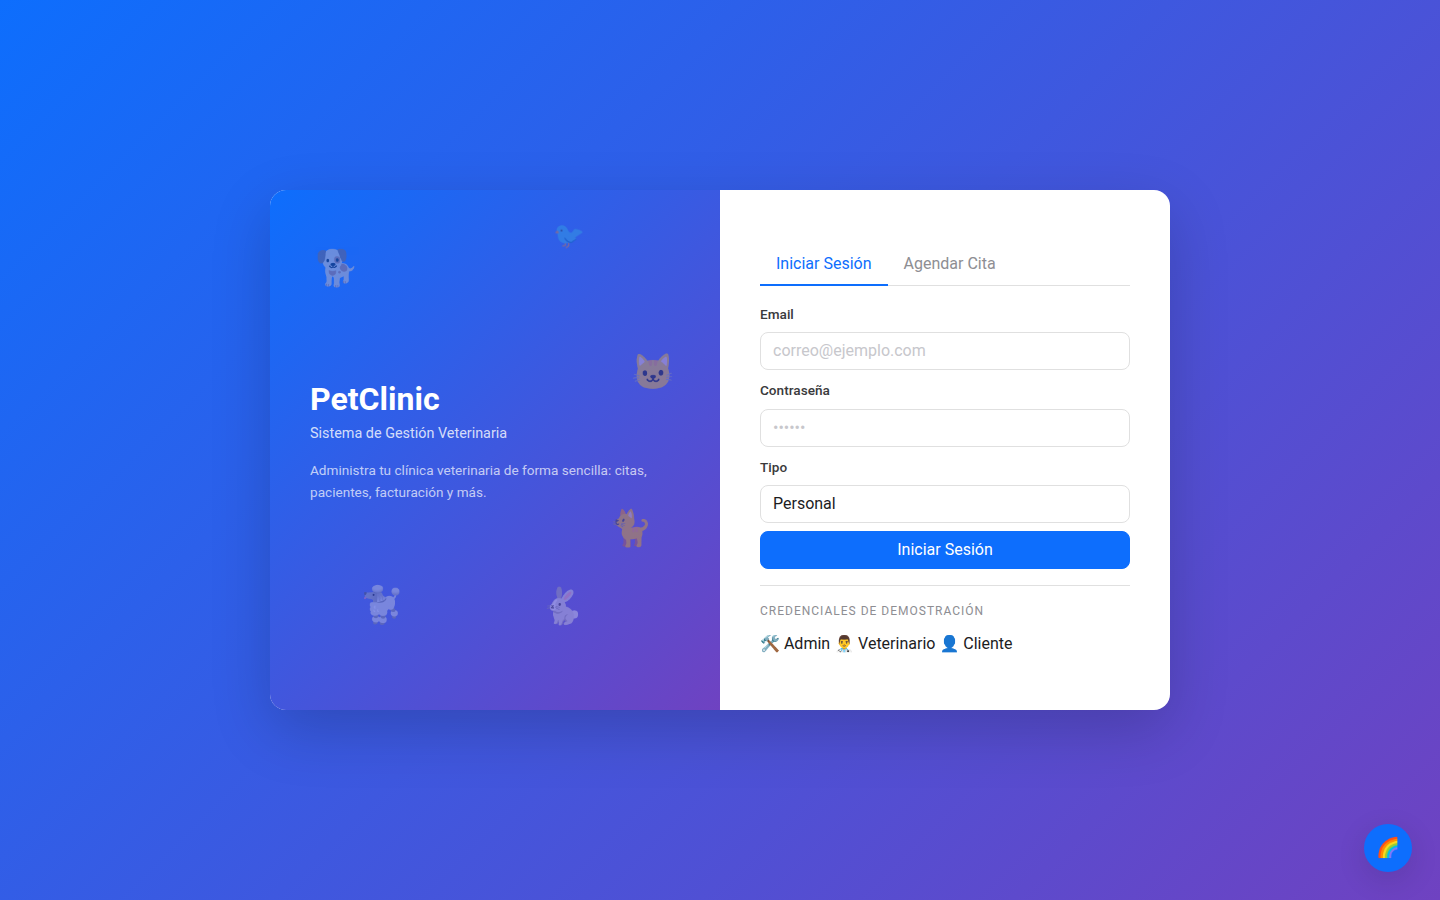
\includegraphics[width=0.8\textwidth]{images/01-login}
    \caption{Pantalla de inicio de sesi\'on con formulario y opci\'on de agenda p\'ublica}
    \label{fig:login}
\end{figure}

\section{Dashboard}

El dashboard muestra 7 tarjetas con estad\'isticas clave del sistema en tiempo real: total de clientes, mascotas, veterinarios, citas hoy, citas pendientes, pacientes hospitalizados y medicamentos con stock bajo. Los datos se cargan mediante \texttt{apiGet('/api/medico/dashboard')} al entrar a la secci\'on.

\begin{figure}[H]
    \centering
    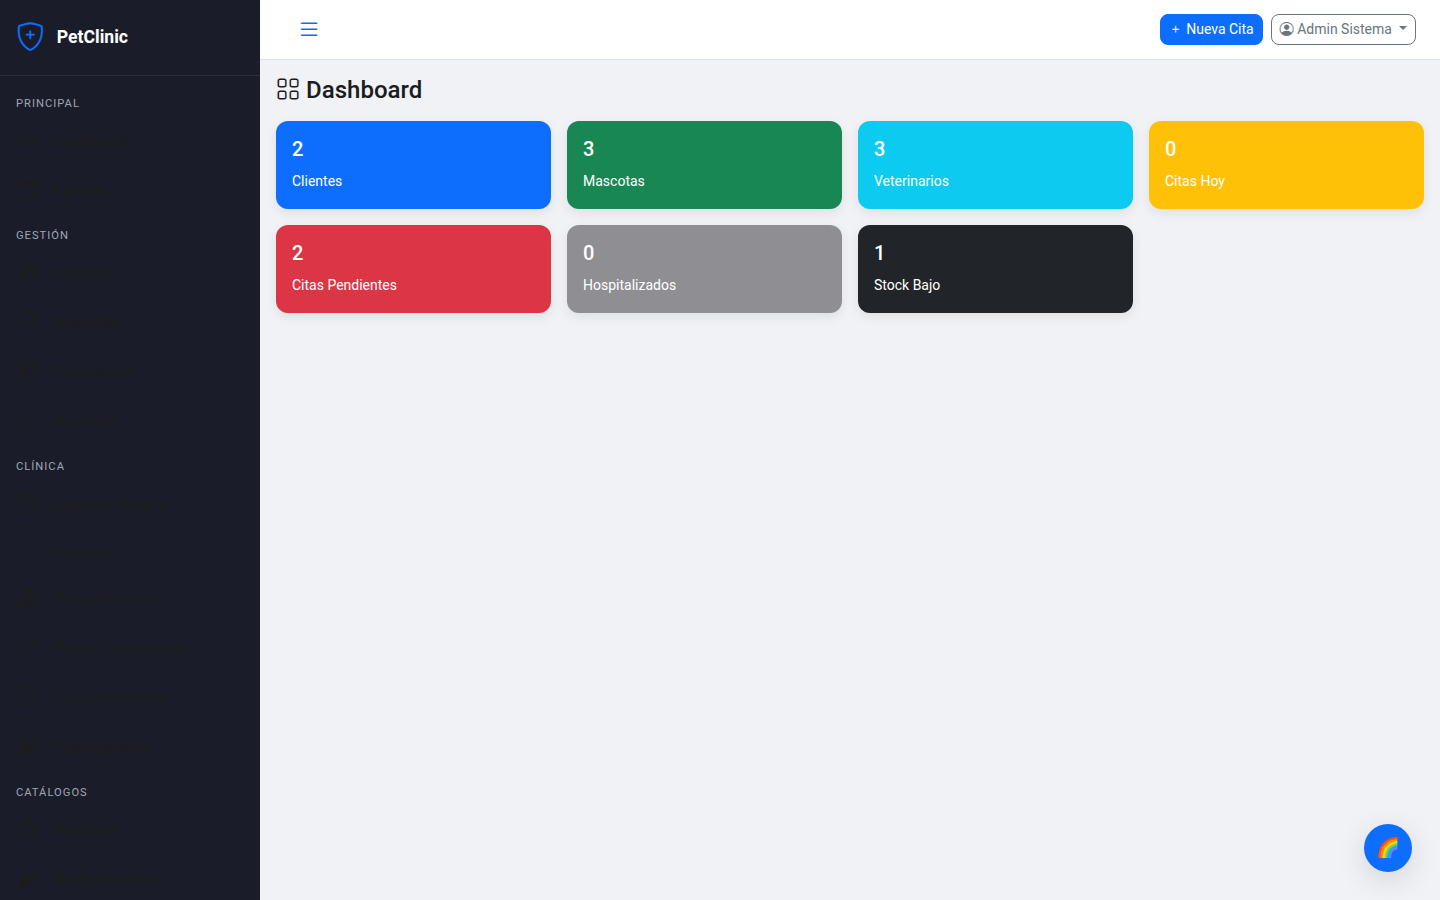
\includegraphics[width=0.9\textwidth]{images/02-dashboard}
    \caption{Dashboard principal con 7 tarjetas de estad\'isticas}
    \label{fig:dashboard2}
\end{figure}

\section{Agenda de Citas}

Utiliza FullCalendar 6 con vistas mensual, semanal y diaria. Soporta arrastrar y soltar para reprogramar citas, codificaci\'on por colores seg\'un el estado (verde=Completada, azul=Programada, amarillo=Confirmada, rojo=Cancelada), y actualizaciones en tiempo real mediante WebSocket.

\begin{lstlisting}[language=JavaScript, caption=Inicializaci\'on de FullCalendar]
const calendar = new FullCalendar.Calendar(calendarEl, {
    plugins: [dayGridPlugin, timeGridPlugin, interactionPlugin],
    headerToolbar: {
        left: 'prev,next today',
        center: 'title',
        right: 'dayGridMonth,timeGridWeek,timeGridDay'
    },
    editable: true,
    events: function(info, successCallback) {
        apiGet('/api/medico/citas').then(data => {
            successCallback(data.map(cita => ({
                id: cita.id,
                title: cita.mascotaNombre + ' - ' + cita.motivo,
                start: cita.fechaHoraInicio,
                end: cita.fechaHoraFin,
                backgroundColor: coloresEstado[cita.estado],
                extendedProps: { estado: cita.estado }
            })));
        });
    },
    eventDrop: function(info) {
        apiPut('/api/medico/citas/' + info.event.id + '/reprogramar', {
            fechaHoraInicio: info.event.start.toISOString(),
            fechaHoraFin: info.event.end.toISOString()
        });
    }
});
calendar.render();
\end{lstlisting}

\begin{figure}[H]
    \centering
    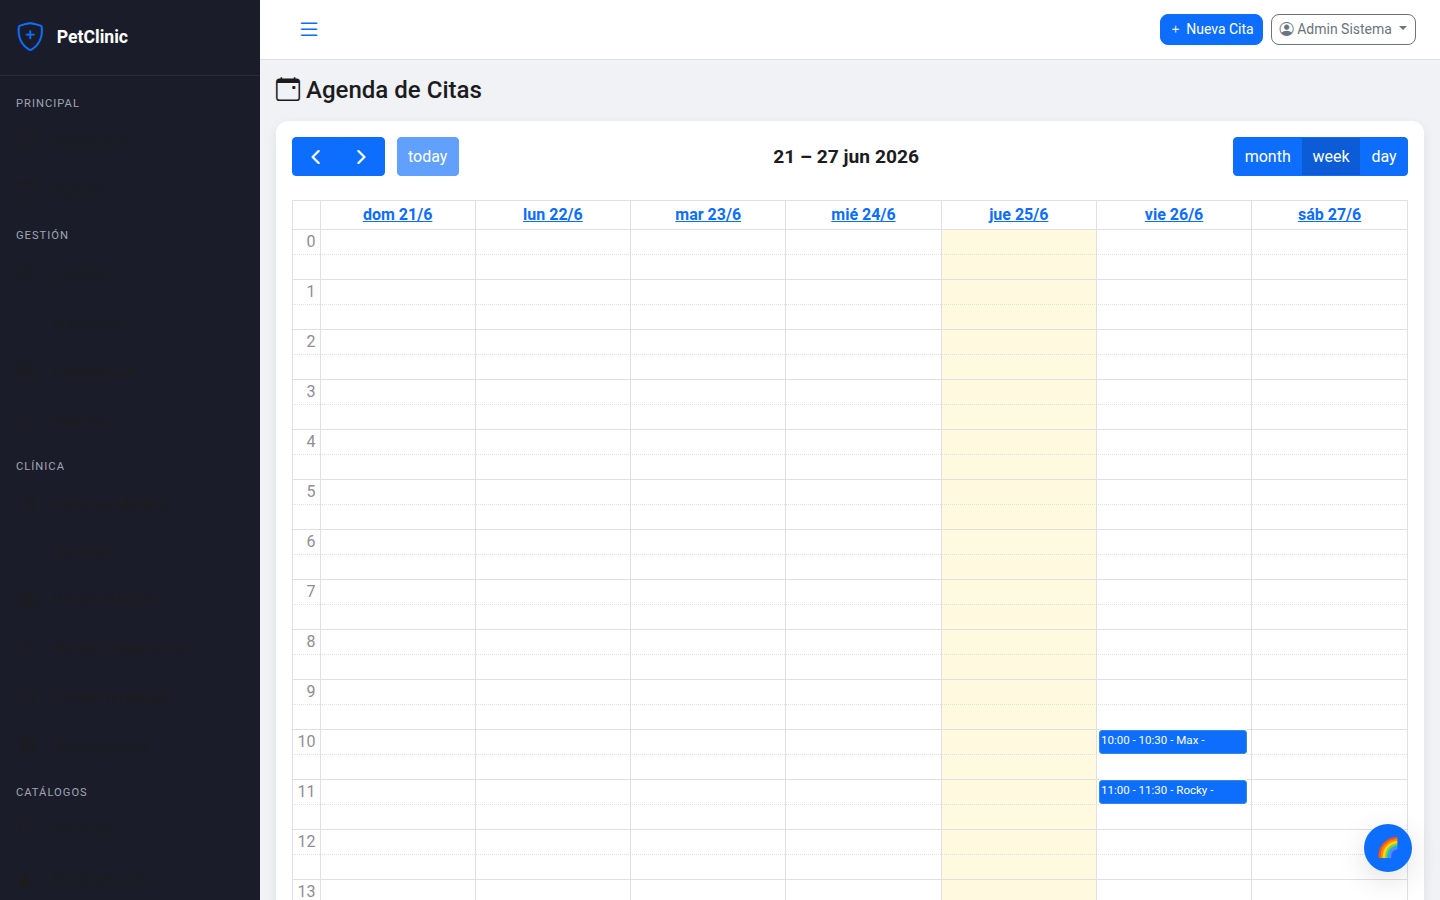
\includegraphics[width=0.9\textwidth]{images/03-agenda}
    \caption{Agenda de citas con FullCalendar en vista mensual}
    \label{fig:agenda}
\end{figure}

\begin{figure}[H]
    \centering
    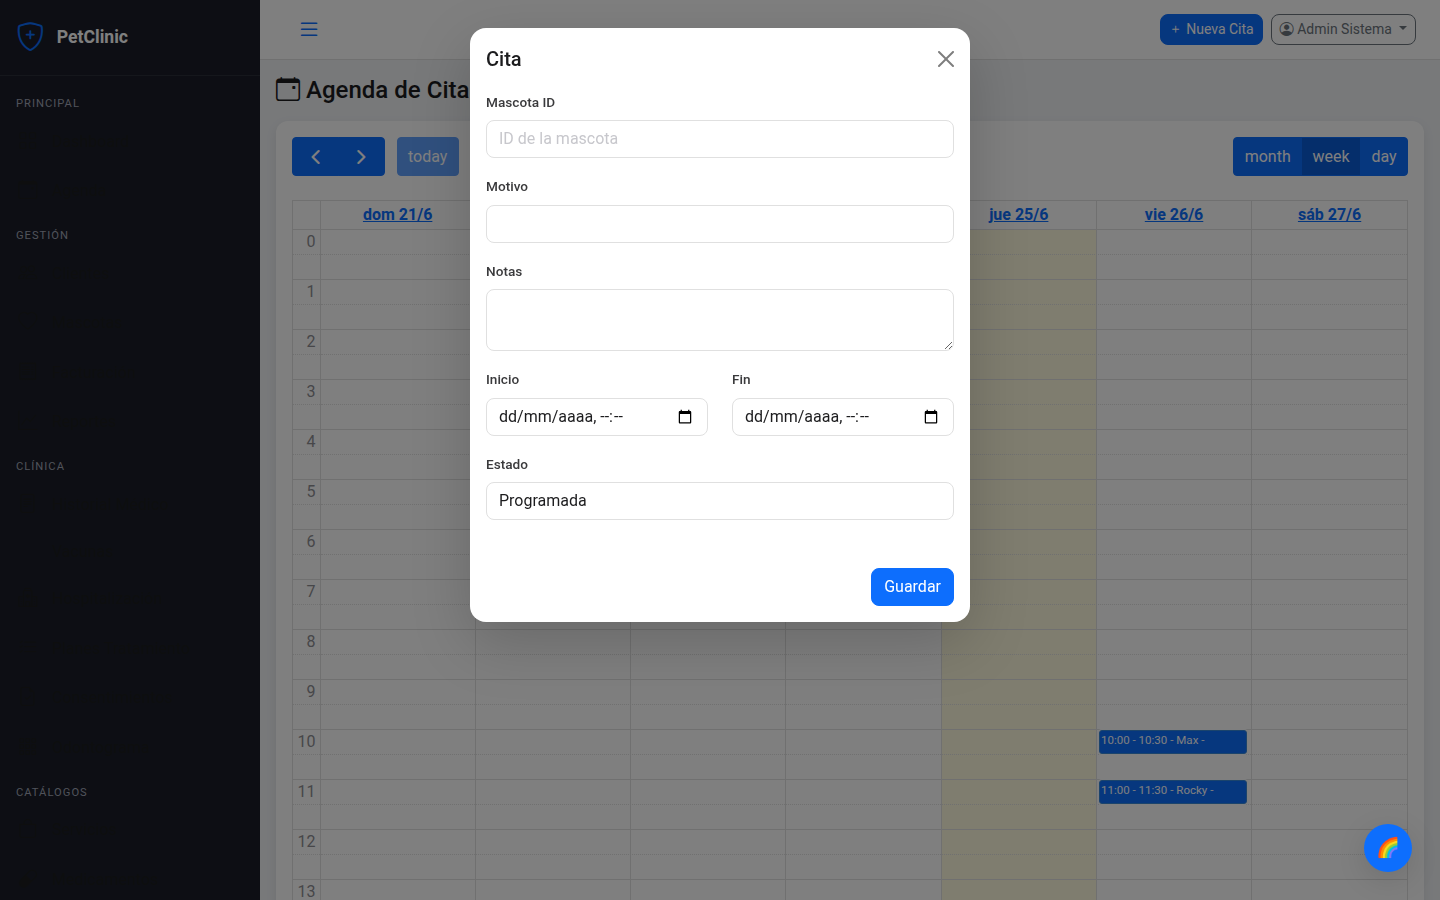
\includegraphics[width=0.6\textwidth]{images/20-modal-cita}
    \caption{Modal de creaci\'on/edici\'on de cita}
    \label{fig:modal-cita}
\end{figure}

\section{Gesti\'on de Clientes y Mascotas}

El m\'odulo de clientes presenta una tabla con b\'usqueda de texto libre, CRUD completo y vista detallada con mascotas asociadas. El m\'odulo de mascotas incluye informaci\'on detallada como especie, raza, peso, alergias y condiciones m\'edicas. Ambos m\'odulos utilizan modales Bootstrap para los formularios de creaci\'on/edici\'on.

\begin{figure}[H]
    \centering
    \begin{subfigure}[b]{0.48\textwidth}
        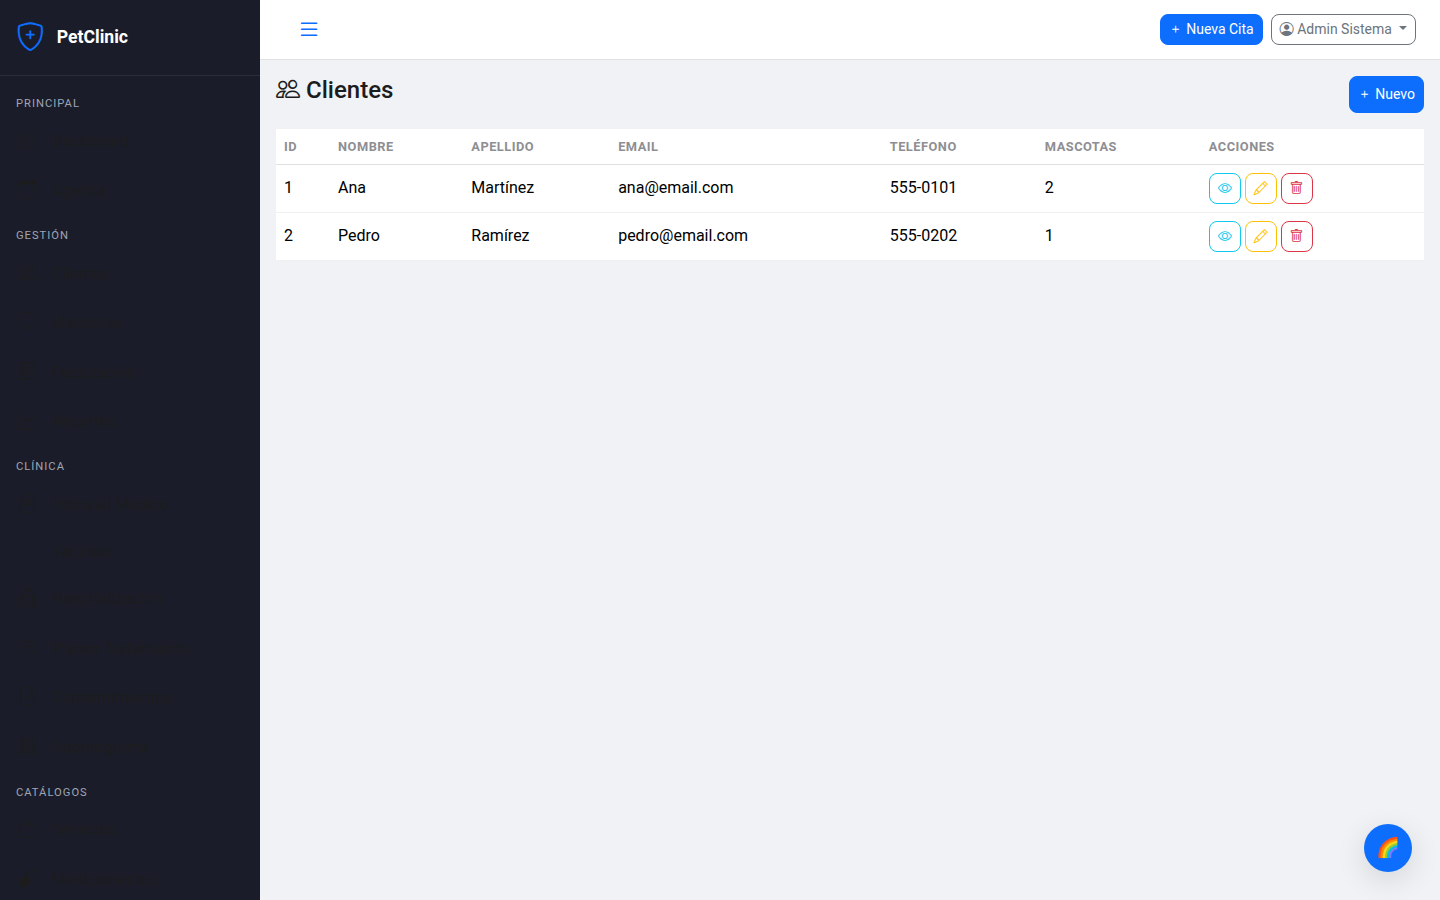
\includegraphics[width=\textwidth]{images/04-clientes}
        \caption{Listado de clientes con b\'usqueda}
    \end{subfigure}
    \hfill
    \begin{subfigure}[b]{0.48\textwidth}
        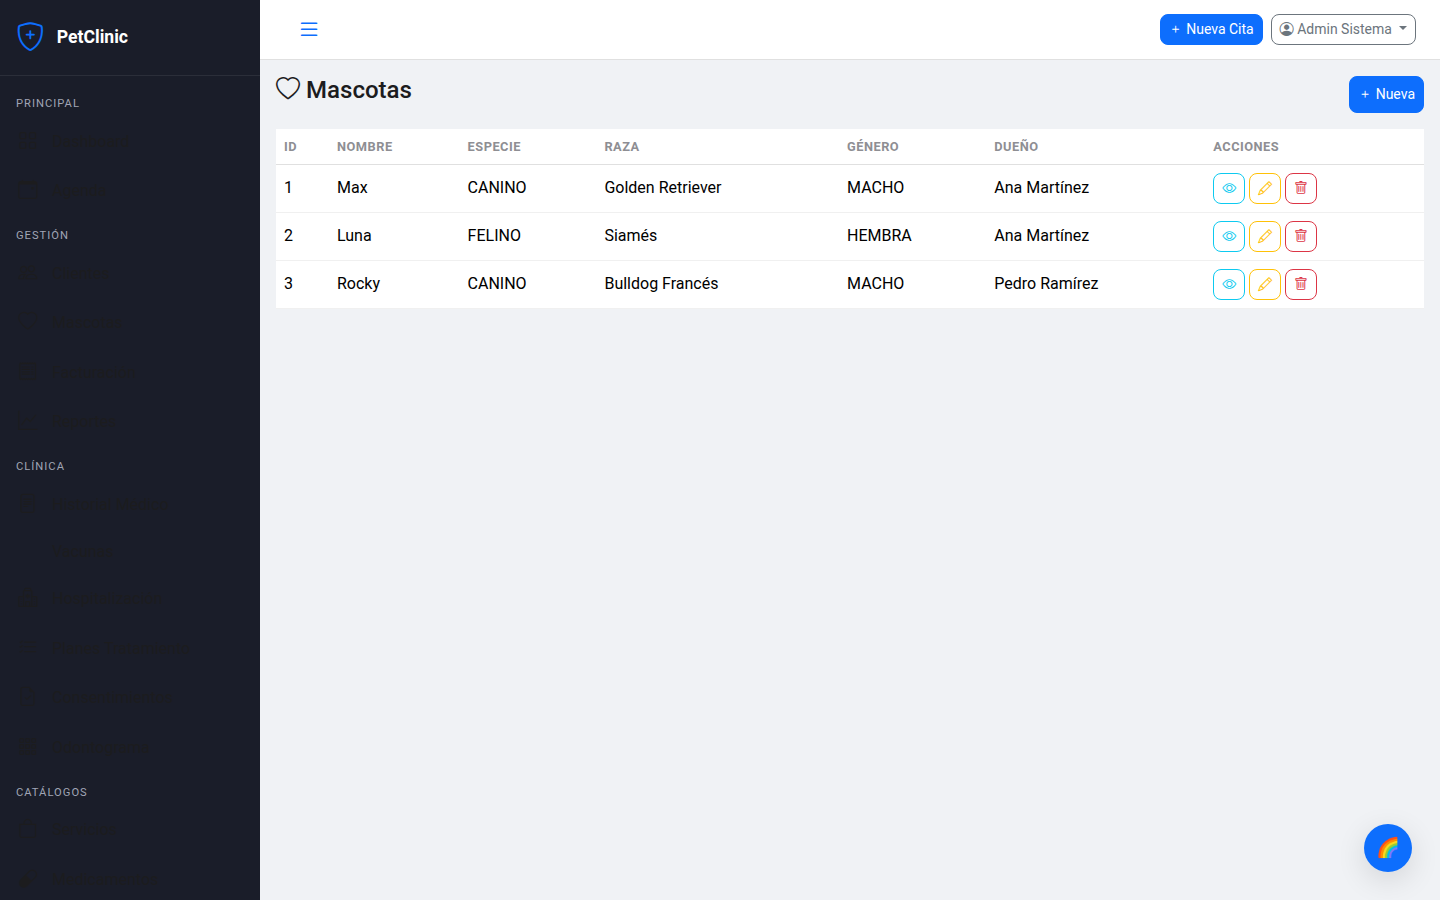
\includegraphics[width=\textwidth]{images/05-mascotas}
        \caption{Listado de mascotas por cliente}
    \end{subfigure}
    \caption{M\'odulos de clientes y mascotas}
    \label{fig:crm}
\end{figure}

\section{Facturaci\'on}

El m\'odulo de facturaci\'on permite crear facturas con items din\'amicos (servicios y medicamentos), c\'alculo autom\'atico de subtotales y totales, descuento autom\'atico de stock, registro de pagos parciales y generaci\'on de PDF con iText 7.

\begin{lstlisting}[language=JavaScript, caption=Creaci\'on de factura con items din\'amicos]
async function guardarFactura() {
    const detalles = [];
    document.querySelectorAll('#detalles-factura .item-row').forEach(row => {
        const tipoItem = row.querySelector('.tipo-item').value;
        const servicioId = row.querySelector('.servicio-id')?.value;
        const medicamentoId = row.querySelector('.medicamento-id')?.value;
        const cantidad = parseInt(row.querySelector('.cantidad').value);
        const precio = parseFloat(row.querySelector('.precio-unitario').value);

        detalles.push({
            tipoItem, servicioId, medicamentoId,
            descripcionLinea: row.querySelector('.descripcion').value,
            cantidad, precioUnitario: precio
        });
    });

    const data = await apiPost('/api/medico/facturas', {
        clienteId: parseInt(document.getElementById('cliente-factura').value),
        detalles: detalles
    });

    toast('Factura creada exitosamente', 'success');
    cargarFacturas();
}
\end{lstlisting}

\begin{figure}[H]
    \centering
    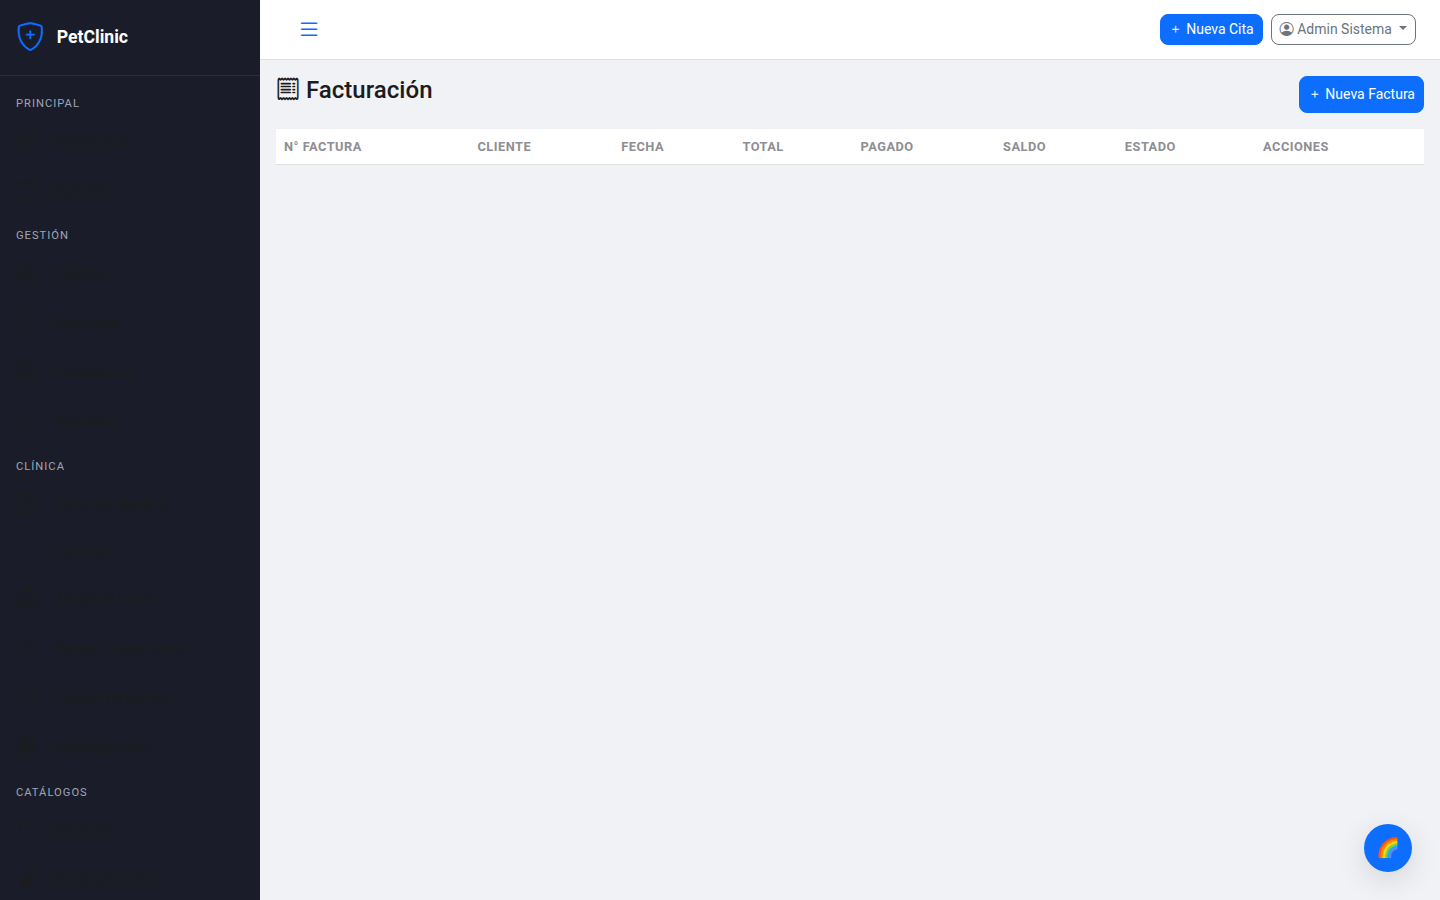
\includegraphics[width=0.9\textwidth]{images/06-facturacion}
    \caption{M\'odulo de facturaci\'on con items din\'amicos}
    \label{fig:facturacion}
\end{figure}

\section{Reportes}

Utiliza Chart.js para mostrar gr\'aficos de ingresos por per\'iodo con opci\'on de descarga en Excel generado con Apache POI en el backend.

\begin{lstlisting}[language=JavaScript, caption=Renderizado de gr\'afico de ingresos con Chart.js]
async function cargarReporte() {
    const data = await apiGet('/api/medico/reportes/ingresos' +
        '?inicio=' + document.getElementById('fecha-inicio').value +
        '&fin=' + document.getElementById('fecha-fin').value);

    new Chart(document.getElementById('chart-ingresos'), {
        type: 'bar',
        data: {
            labels: data.map(d => d.fecha),
            datasets: [{
                label: 'Ingresos ($)',
                data: data.map(d => d.total),
                backgroundColor: 'rgba(54, 162, 235, 0.5)',
                borderColor: 'rgba(54, 162, 235, 1)',
                borderWidth: 1
            }]
        },
        options: {
            responsive: true,
            plugins: {
                legend: { display: true },
                tooltip: { callbacks: {
                    label: ctx => '$' + ctx.parsed.y.toFixed(2)
                }}
            }
        }
    });
}
\end{lstlisting}

\begin{figure}[H]
    \centering
    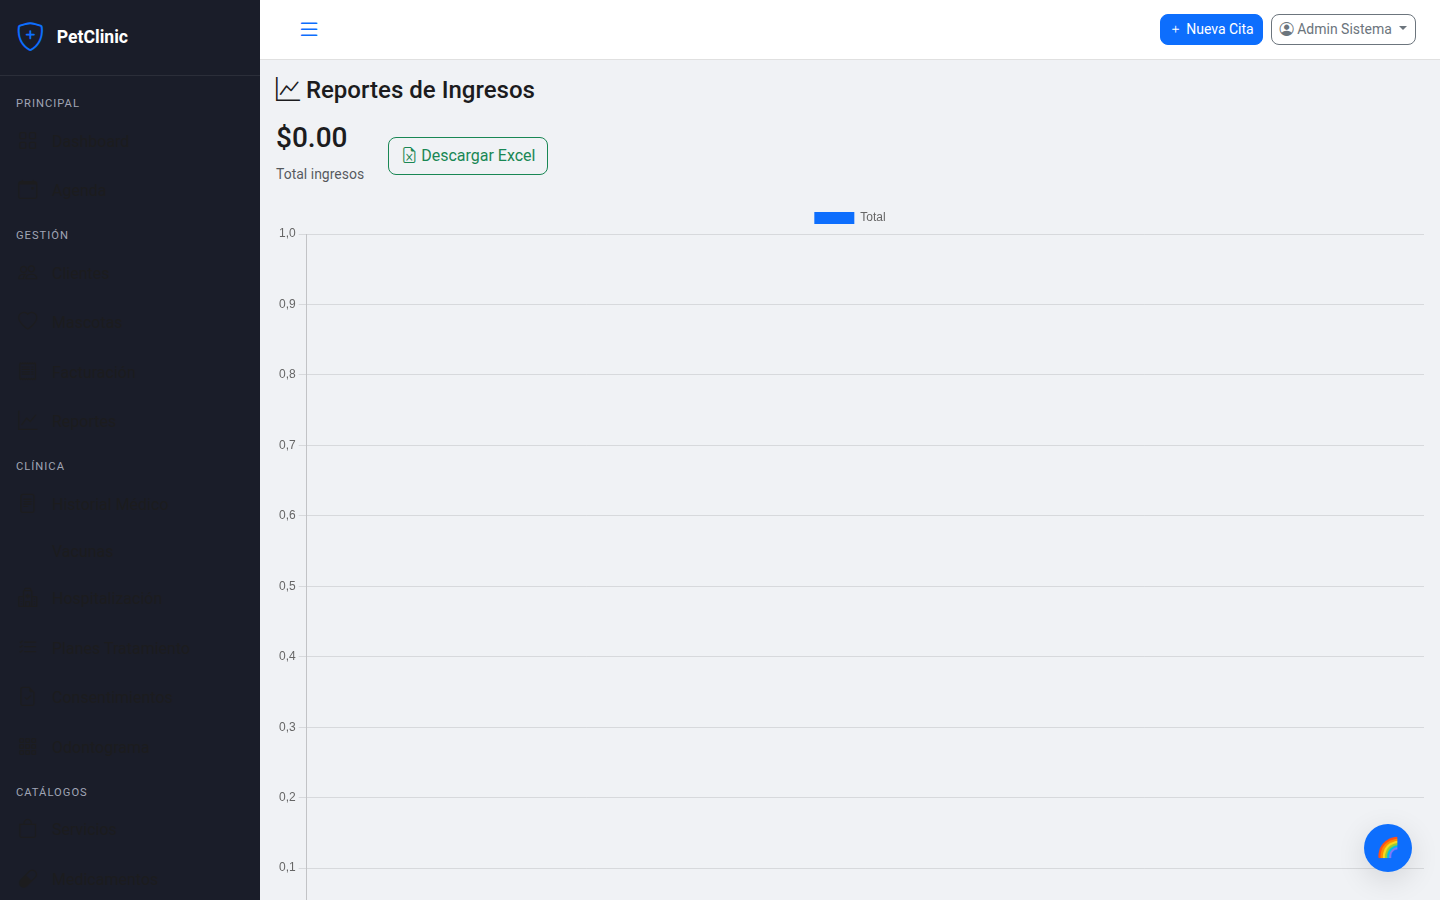
\includegraphics[width=0.9\textwidth]{images/07-reportes}
    \caption{Reportes de ingresos con Chart.js}
    \label{fig:reportes}
\end{figure}

\section{Odontograma Canino}

El odontograma es un diagrama dental interactivo para caninos con 42 dientes numerados seg\'un la f\'ormula dental canina (I 3/3, C 1/1, P 4/4, M 2/3). Permite seleccionar el estado de cada diente (Sano, T\'artaro, Caries, Fractura, Ausente, Periodontal, Obturado, Endodoncia) haciendo clic en el diente correspondiente. El estado se persiste en la base de datos y se pueden tener m\'ultiples odontogramas por mascota (uno por consulta).

\begin{figure}[H]
    \centering
    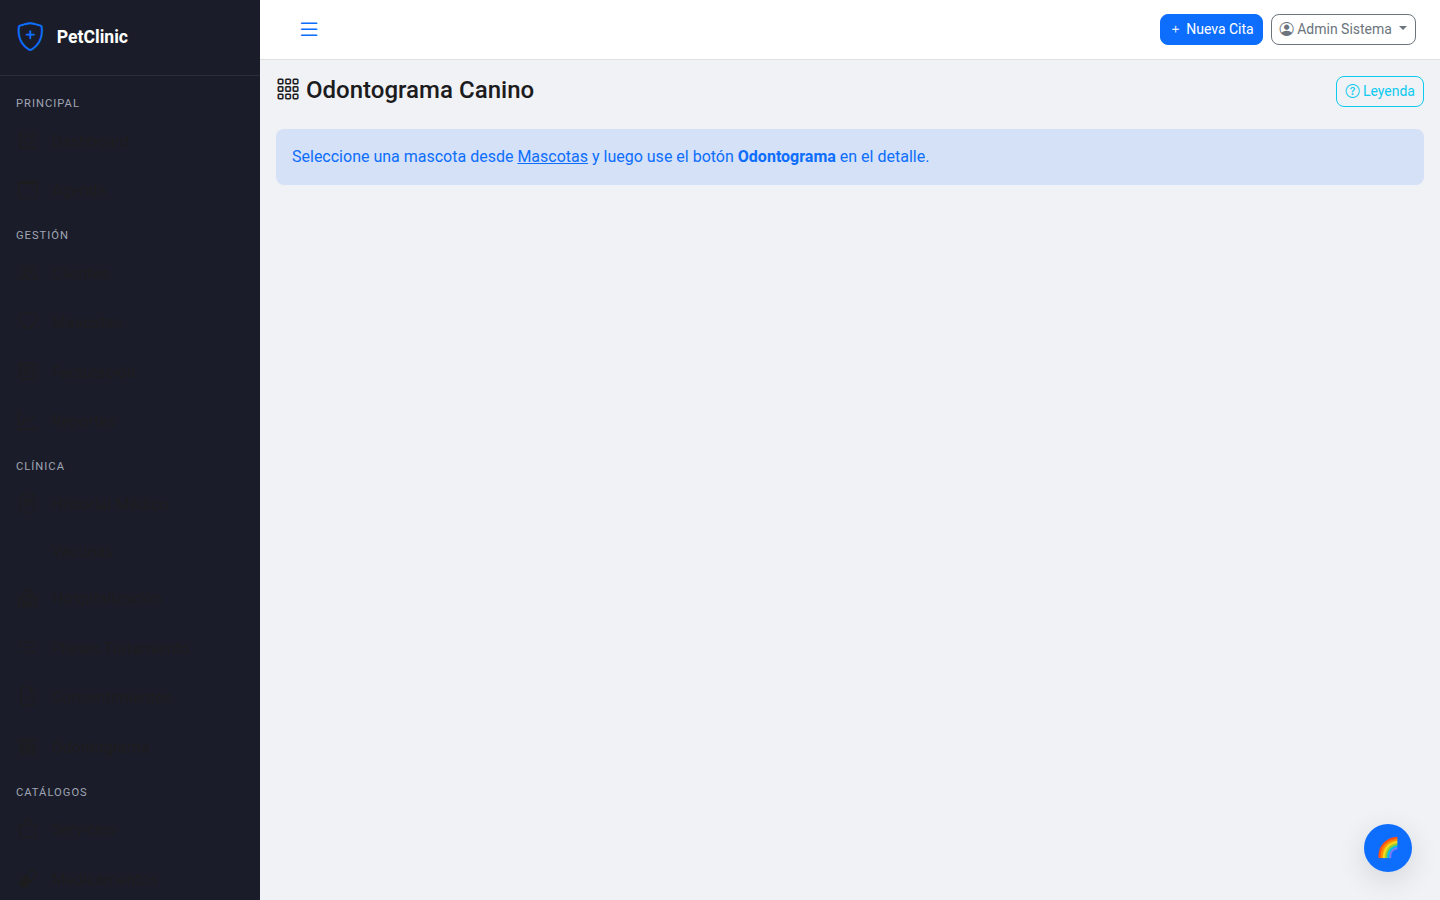
\includegraphics[width=0.9\textwidth]{images/13-odontograma}
    \caption{Odontograma canino interactivo con 42 dientes y 8 estados}
    \label{fig:odontograma}
\end{figure}

\section{Portal del Cliente}

El portal del cliente permite a los due\~nos de mascotas consultar sus citas, facturas e historial m\'edico de manera autogestionada, sin necesidad de contacto con el personal de la cl\'inica.

\begin{figure}[H]
    \centering
    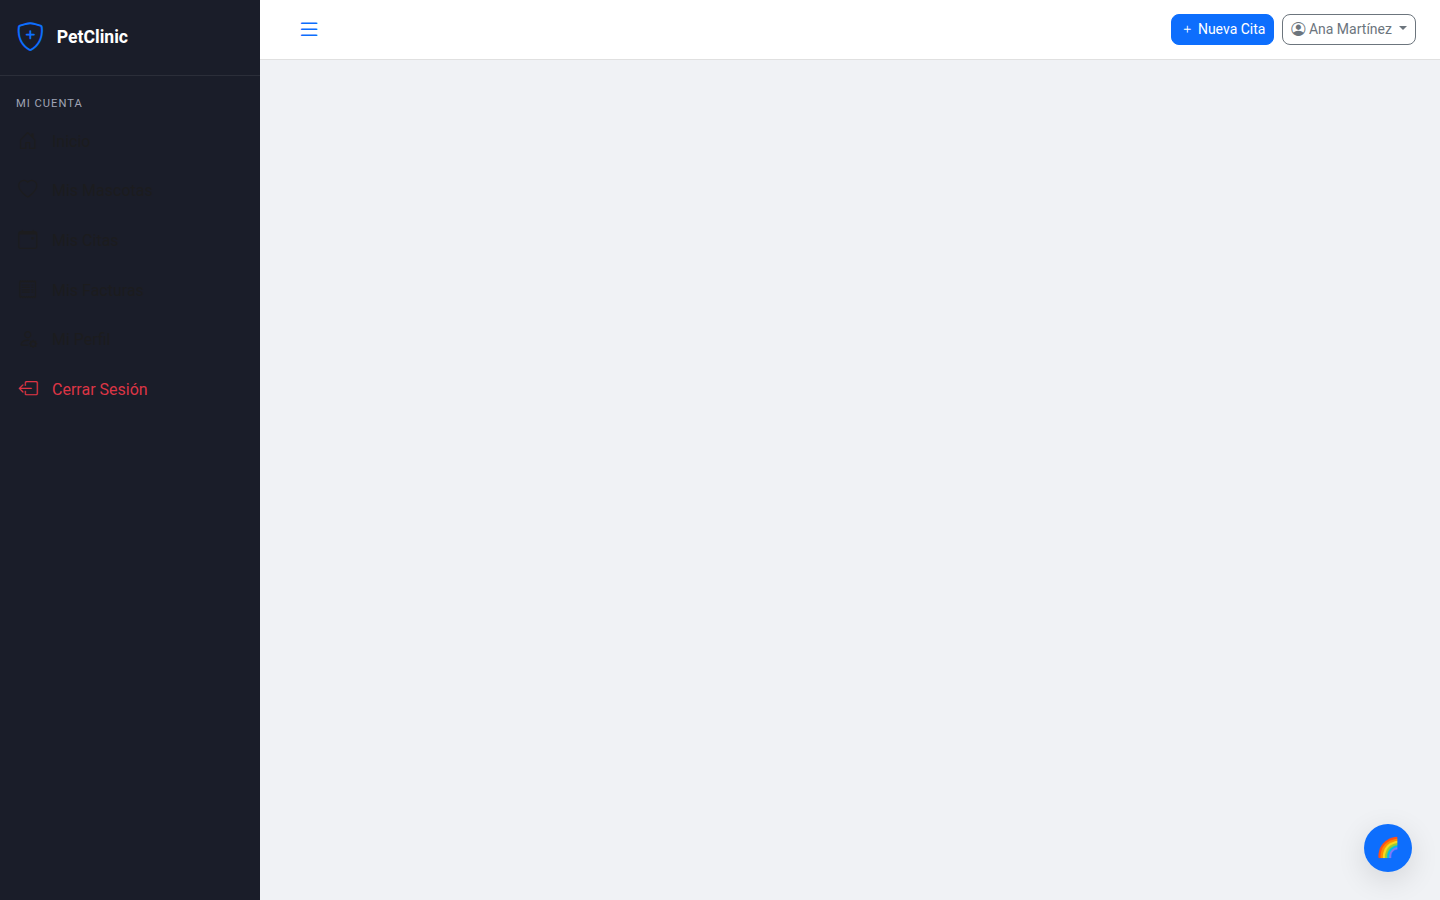
\includegraphics[width=0.9\textwidth]{images/19-portal-cliente}
    \caption{Portal del cliente con citas, mascotas y facturas}
    \label{fig:portal}
\end{figure}

\section{Sistema de Temas}

El sistema incluye 8 temas de color que se pueden cambiar en tiempo real sin recargar la p\'agina mediante el bot\'on flotante en la esquina inferior derecha:

\begin{itemize}
    \item \textbf{Light:} Tema claro predeterminado con fondo blanco y texto oscuro.
    \item \textbf{Dark:} Modo oscuro con fondo \#1a1a2e y texto claro.
    \item \textbf{Terracota:} Tonos tierra c\'alidos con acentos en terracota.
    \item \textbf{Blue Pro:} Azul profesional corporativo.
    \item \textbf{Pink:} Acento rosa para interfaces m\'as suaves.
    \item \textbf{Purple:} Acento p\'urpura con tonos violeta.
    \item \textbf{Olive:} Tonos verdes oliva.
    \item \textbf{Burn (Sunset):} \'Ambar oscuro con degradados de atardecer.
\end{itemize}

Los temas se implementan mediante variables CSS (\textit{Custom Properties}) y se persisten en \texttt{localStorage}. Al cambiar de tema, se actualiza la variable \texttt{data-theme} en el elemento \texttt{<html>} y FullCalendar se refresca autom\'aticamente.

\section{API Cliente (api.js)}

El m\'odulo \texttt{api.js} encapsula toda la comunicaci\'on con el backend HTTP mediante fetch API con manejo centralizado de errores:

\begin{lstlisting}[language=JavaScript, caption=Cliente HTTP con autenticaci\'on JWT]
const API_BASE = '/api';

function getToken() { return localStorage.getItem('vet_token'); }
function getUser() { return JSON.parse(localStorage.getItem('vet_user')||'{}'); }

function authHeaders() {
    return {
        'Content-Type': 'application/json',
        'Authorization': 'Bearer ' + getToken()
    };
}

async function apiGet(path) {
    const res = await fetch(API_BASE + path, { headers: authHeaders() });
    if (!res.ok) {
        const err = await res.json().catch(() => ({}));
        throw new Error(err.error || 'Error ' + res.status);
    }
    return res.json();
}

async function apiPost(path, body) {
    const res = await fetch(API_BASE + path, {
        method: 'POST', headers: authHeaders(),
        body: JSON.stringify(body)
    });
    if (!res.ok) throw new Error((await res.json()).error);
    return res.json();
}

async function apiPut(path, body) {
    const res = await fetch(API_BASE + path, {
        method: 'PUT', headers: authHeaders(),
        body: JSON.stringify(body)
    });
    if (!res.ok) throw new Error((await res.json()).error);
    return res.json();
}

async function apiDelete(path) {
    const res = await fetch(API_BASE + path, {
        method: 'DELETE', headers: authHeaders()
    });
    if (!res.ok) throw new Error((await res.json()).error);
    return res.json();
}

function fmt(num) { return '$' + Number(num||0).toFixed(2); }

function toast(msg, type) {
    const el = document.createElement('div');
    el.className = 'toast show position-fixed bottom-0 end-0 m-3';
    el.innerHTML = '<div class="toast-header bg-' + type + ' text-white">'
        + '<strong>' + type.toUpperCase() + '</strong>'
        + '<button type="button" class="btn-close btn-close-white" '
        + 'data-bs-dismiss="toast"></button></div>'
        + '<div class="toast-body">' + msg + '</div>';
    document.body.appendChild(el);
    setTimeout(() => el.remove(), 3000);
}
\end{lstlisting}

\chapter{Seguridad}

\section{Autenticaci\'on JWT}

El sistema utiliza JSON Web Tokens (JWT) para la autenticaci\'on stateless. La implementaci\'on se compone de cuatro clases principales que trabajan en conjunto para validar cada petici\'on HTTP.

\subsection{JwtTokenProvider}

Genera y valida tokens JWT firmados con HMAC-SHA384, incluyendo informaci\'on del usuario en los claims del token.

\begin{lstlisting}[language=Java, caption=JwtTokenProvider: generaci\'on y validaci\'on de tokens]
@Component
public class JwtTokenProvider {
    @Value("${app.jwt.secret}")
    private String jwtSecret;

    @Value("${app.jwt.expiration}")
    private long jwtExpiration;

    private Key getSigningKey() {
        return Keys.hmacShaKeyFor(jwtSecret.getBytes());
    }

    public String generateToken(String email, String rol, Long userId) {
        Date now = new Date();
        Date expiry = new Date(now.getTime() + jwtExpiration);

        return Jwts.builder()
            .subject(email)
            .claim("rol", rol)
            .claim("userId", userId)
            .issuedAt(now)
            .expiration(expiry)
            .signWith(getSigningKey())
            .compact();
    }

    public boolean validateToken(String token) {
        try {
            Jwts.parser().verifyWith(getSigningKey()).build()
                .parseSignedClaims(token);
            return true;
        } catch (JwtException | IllegalArgumentException e) {
            return false;
        }
    }

    public String getEmailFromToken(String token) {
        return Jwts.parser().verifyWith(getSigningKey()).build()
            .parseSignedClaims(token).getPayload().getSubject();
    }

    public String getRolFromToken(String token) {
        return Jwts.parser().verifyWith(getSigningKey()).build()
            .parseSignedClaims(token).getPayload()
            .get("rol", String.class);
    }

    public Long getUserIdFromToken(String token) {
        return Jwts.parser().verifyWith(getSigningKey()).build()
            .parseSignedClaims(token).getPayload()
            .get("userId", Long.class);
    }
}
\end{lstlisting}

\begin{itemize}
    \item \textbf{Claims:} subject (email del usuario), rol (ADMIN/VETERINARIO/RECEPCIONISTA/CLIENTE), userId.
    \item \textbf{Firma:} HMAC-SHA384 con clave secreta configurable v\'ia \texttt{JWT\_SECRET}.
    \item \textbf{Expiraci\'on:} 30 minutos (configurable v\'ia \texttt{app.jwt.expiration}).
\end{itemize}

\subsection{JwtAuthFilter}

Filtro que intercepta todas las peticiones HTTP entrantes y valida el token JWT presente en el header \texttt{Authorization}. Si el token es v\'alido, establece el contexto de seguridad con los roles del usuario.

\begin{lstlisting}[language=Java, caption=Filtro de autenticaci\'on JWT]
@Component
public class JwtAuthFilter extends OncePerRequestFilter {

    @Autowired private JwtTokenProvider jwtProvider;

    @Override
    protected void doFilterInternal(HttpServletRequest request,
            HttpServletResponse response, FilterChain chain)
            throws ServletException, IOException {
        String header = request.getHeader("Authorization");

        if (header != null && header.startsWith("Bearer ")) {
            String token = header.substring(7);

            if (jwtProvider.validateToken(token)) {
                String email = jwtProvider.getEmailFromToken(token);
                String rol = jwtProvider.getRolFromToken(token);
                Long userId = jwtProvider.getUserIdFromToken(token);

                UsernamePasswordAuthenticationToken auth =
                    new UsernamePasswordAuthenticationToken(
                        email, userId,
                        List.of(new SimpleGrantedAuthority("ROLE_" + rol)));

                SecurityContextHolder.getContext().setAuthentication(auth);
            }
        }
        chain.doFilter(request, response);
    }
}
\end{lstlisting}

\section{Control de Acceso por Roles}

\subsection{SecurityConfig}

Configura las reglas de acceso basadas en roles mediante \texttt{SecurityFilterChain}:

\begin{itemize}
    \item \textbf{Endpoints p\'ublicos:} \texttt{/api/auth/**}, \texttt{/api/public/**}, \texttt{/api/pagos/stripe/webhook}, \texttt{/ws/**}, recursos est\'aticos.
    \item \textbf{ADMIN:} Acceso completo a todos los endpoints, incluyendo administraci\'on de usuarios y auditor\'ia.
    \item \textbf{VETERINARIO:} CRUD cl\'inico completo (citas, facturas, historial, vacunas, hospitalizaci\'on).
    \item \textbf{RECEPCIONISTA:} S\'olo lectura en la mayor\'ia de recursos; puede crear clientes y citas.
    \item \textbf{CLIENTE:} S\'olo acceso a \texttt{/api/portal/**} (perfil, citas, facturas, mascotas).
\end{itemize}

\begin{lstlisting}[language=Java, caption=Configuraci\'on de seguridad con reglas de acceso]
@Bean
public SecurityFilterChain filterChain(HttpSecurity http) throws Exception {
    http
        .cors(cors -> cors.configurationSource(corsConfig()))
        .csrf(csrf -> csrf.disable())
        .sessionManagement(sm ->
            sm.sessionCreationPolicy(SessionCreationPolicy.STATELESS))
        .authorizeHttpRequests(auth -> auth
            .requestMatchers("/api/auth/**", "/api/public/**").permitAll()
            .requestMatchers("/api/pagos/stripe/webhook").permitAll()
            .requestMatchers("/ws/**").permitAll()
            .requestMatchers("/api/admin/**").hasRole("ADMIN")
            .requestMatchers("/api/admin/auditoria")
                .hasAnyRole("ADMIN", "VETERINARIO")
            .requestMatchers(GET, "/api/medico/**")
                .hasAnyRole("ADMIN", "VETERINARIO", "RECEPCIONISTA")
            .requestMatchers("/api/medico/**")
                .hasAnyRole("ADMIN", "VETERINARIO")
            .requestMatchers("/api/portal/**").hasRole("CLIENTE")
            .anyRequest().authenticated()
        )
        .addFilterBefore(jwtAuthFilter,
            UsernamePasswordAuthenticationFilter.class);
    return http.build();
}
\end{lstlisting}

\section{CustomUserDetailsService}

Implementa \texttt{UserDetailsService} para cargar usuarios desde la base de datos. Soporta dos tipos de autenticaci\'on:

\begin{itemize}
    \item \textbf{Personal:} Busca en la tabla \texttt{veterinarios} (admin, veterinarios, recepcionistas). Usa \texttt{VeterinarioRepository.findByEmail()}.
    \item \textbf{Cliente:} Busca en la tabla \texttt{clientes} donde \texttt{portalActivo = true}. Usa \texttt{ClienteRepository.findByPortalEmail()}.
\end{itemize}

\begin{lstlisting}[language=Java, caption=CustomUserDetailsService]
@Override
public UserDetails loadUserByUsername(String username)
        throws UsernameNotFoundException {
    // Intentar como veterinario (personal)
    Optional<Veterinario> vet = veterinarioRepo.findByEmail(username);
    if (vet.isPresent()) {
        Veterinario v = vet.get();
        if (!v.getActivo()) {
            throw new DisabledException("Usuario desactivado");
        }
        return new User(v.getEmail(), v.getPasswordHash(),
            List.of(new SimpleGrantedAuthority("ROLE_" + v.getRol().name())));
    }

    // Intentar como cliente
    Optional<Cliente> cli = clienteRepo.findByPortalEmail(username);
    if (cli.isPresent()) {
        Cliente c = cli.get();
        if (!c.getPortalActivo()) {
            throw new DisabledException("Portal desactivado");
        }
        return new User(c.getPortalEmail(), c.getPortalPasswordHash(),
            List.of(new SimpleGrantedAuthority("ROLE_CLIENTE")));
    }

    throw new UsernameNotFoundException(
        "Usuario no encontrado: " + username);
}
\end{lstlisting}

\section{Auditor\'ia}

Cada operaci\'on CRUD importante registra un log de auditor\'ia con la siguiente informaci\'on:

\begin{itemize}
    \item Acci\'on realizada (CREATE, UPDATE, DELETE).
    \item Entidad afectada y su ID.
    \item Descripci\'on detallada de la operaci\'on.
    \item ID y email del veterinario que realiz\'o la acci\'on.
    \item Direcci\'on IP del cliente (extra\'ida del header \texttt{X-Forwarded-For} o \texttt{getRemoteAddr()}).
    \item Fecha y hora exacta del evento.
\end{itemize}

\begin{lstlisting}[language=Java, caption=Ejemplo de registro de auditor\'ia]
public void log(String accion, String entidad, Long entidadId,
        String descripcion, Long vetId, String vetEmail) {
    AuditLog log = new AuditLog();
    log.setAccion(accion);
    log.setEntidad(entidad);
    log.setEntidadId(entidadId);
    log.setDescripcion(descripcion);
    log.setVeterinarioId(vetId);
    log.setVeterinarioEmail(vetEmail);
    log.setDireccionIp(obtenerDireccionIp());
    log.setFechaAccion(LocalDateTime.now());
    auditLogRepo.save(log);
}
\end{lstlisting}

\begin{figure}[H]
    \centering
    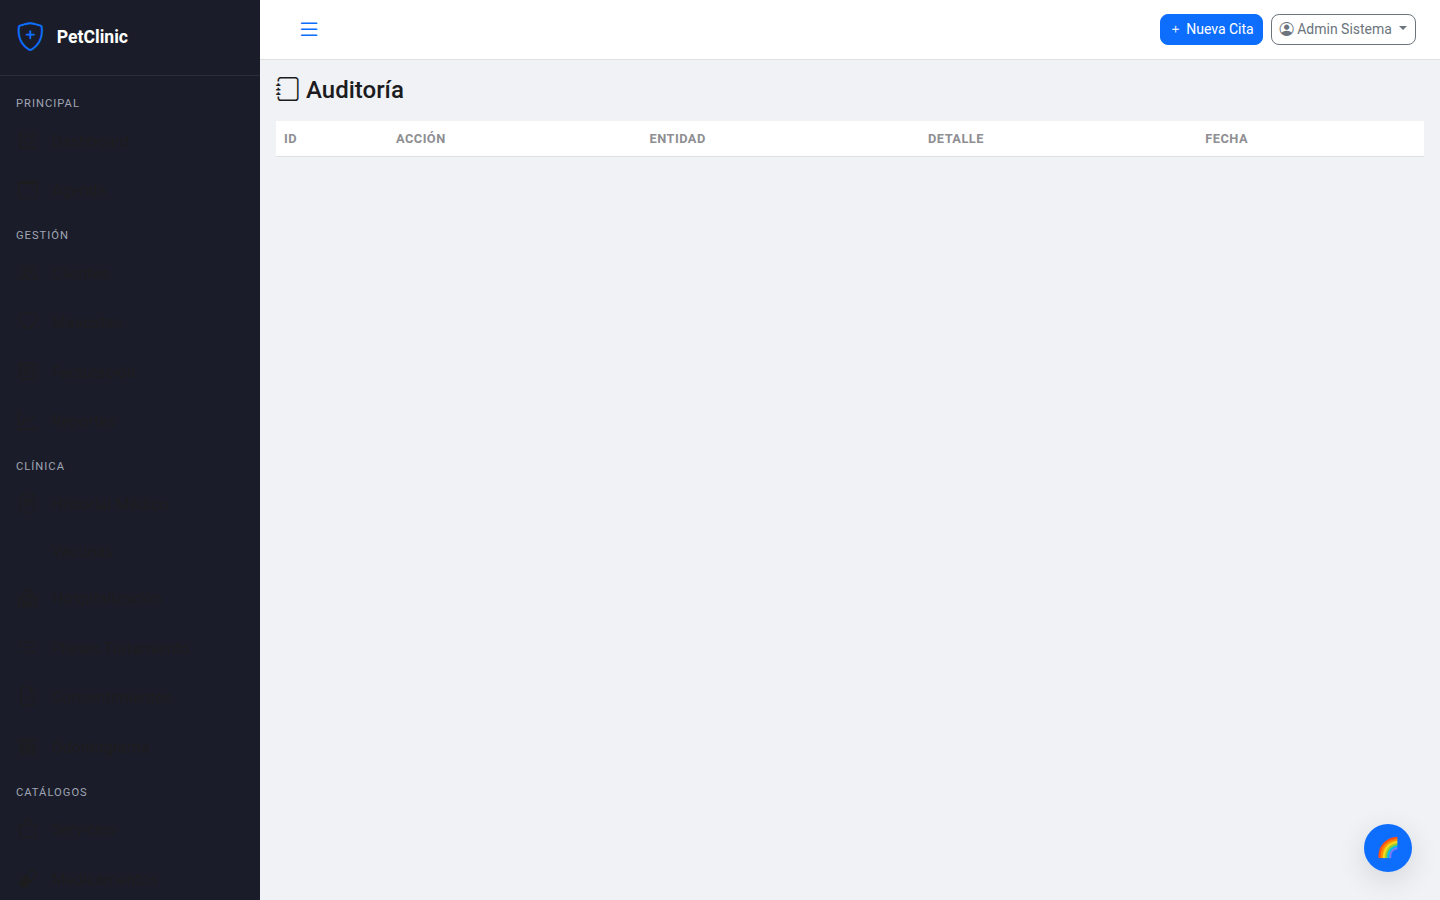
\includegraphics[width=0.9\textwidth]{images/17-auditoria}
    \caption{Registro de auditor\'ia con detalle de acciones por usuario}
    \label{fig:auditoria}
\end{figure}

\section{Protecci\'on de Contrase\~nas}

Todas las contrase\~nas se almacenan usando BCrypt mediante \texttt{BCryptPasswordEncoder} de Spring Security, con factor de costo 10 (10 rondas de hashing). El \texttt{PasswordEncoder} se define como un bean en \texttt{SecurityConfig}:

\begin{lstlisting}[language=Java]
@Bean
public PasswordEncoder passwordEncoder() {
    return new BCryptPasswordEncoder();
}
\end{lstlisting}

\section{CORS}

Configuraci\'on que permite peticiones desde cualquier origen para desarrollo, con soporte para credenciales:

\begin{lstlisting}[language=Java, caption=Configuraci\'on CORS]
@Bean
public WebMvcConfigurer corsConfigurer() {
    return new WebMvcConfigurer() {
        @Override
        public void addCorsMappings(CorsRegistry registry) {
            registry.addMapping("/api/**")
                .allowedOriginPatterns("*")
                .allowedMethods("GET", "POST", "PUT", "DELETE", "OPTIONS")
                .allowedHeaders("*")
                .allowCredentials(true);
        }
    };
}
\end{lstlisting}

\section{Protecci\'on CSRF}

CSRF est\'a deshabilitado porque la aplicaci\'on utiliza JWT stateless, lo que hace que los tokens CSRF sean innecesarios. La protecci\'on contra CSRF se logra mediante la validaci\'on del token JWT en cada petici\'on. En producci\'on, se recomienda agregar \texttt{HttpOnly} y \texttt{Secure} a las cookies si se usan, pero dado que el token se almacena en \texttt{localStorage} del navegador, la protecci\'on principal es contra XSS.

\chapter{M\'odulos del Sistema}

\section{Visi\'on General}

PetClinic cuenta con 20 m\'odulos funcionales que cubren todas las \'areas operativas de una cl\'inica veterinaria. Cada m\'odulo consta de su controlador REST, servicio, repositorio y vista en el frontend, siguiendo la arquitectura en capas descrita en el cap\'itulo 2.

\section{M\'odulo de Veterinarios}

Gesti\'on completa del personal de la cl\'inica con roles diferenciados:

\begin{itemize}
    \item CRUD completo de veterinarios (s\'olo administradores).
    \item Roles: ADMIN, VETERINARIO, RECEPCIONISTA.
    \item Gesti\'on de horarios y duraci\'on de turnos.
    \item Activaci\'on/desactivaci\'on de cuentas (\textit{soft delete}).
    \item Cambio de contrase\~na con verificaci\'on de contrase\~na actual.
\end{itemize}

\begin{figure}[H]
    \centering
    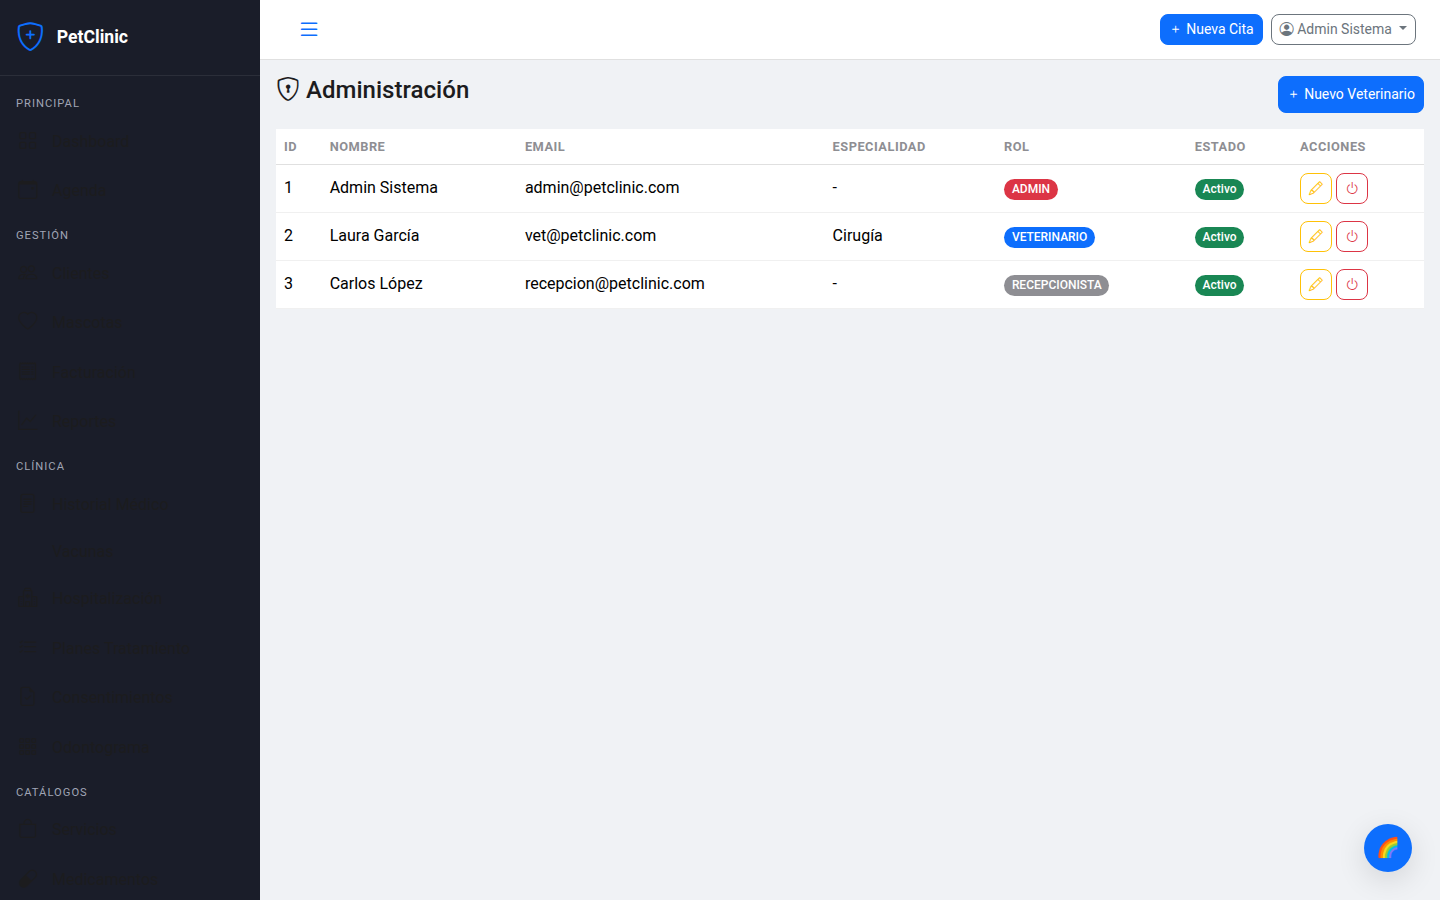
\includegraphics[width=0.9\textwidth]{images/16-admin-veterinarios}
    \caption{Gesti\'on de veterinarios desde el panel de administraci\'on}
    \label{fig:admin}
\end{figure}

\section{M\'odulo de Clientes}

Registro y gesti\'on de due\~nos de mascotas:

\begin{itemize}
    \item Registro con datos de contacto y direcci\'on.
    \item B\'usqueda por nombre, apellido o email.
    \item Portal web para clientes (citas, facturas, historial).
    \item Vista detallada con mascotas asociadas.
\end{itemize}

\section{M\'odulo de Mascotas}

Registro detallado de pacientes con informaci\'on cl\'inica completa:

\begin{itemize}
    \item Informaci\'on completa: especie, raza, color, g\'enero, peso.
    \item Control de alergias y condiciones m\'edicas.
    \item Vista unificada con citas, historial, vacunas y planes.
    \item Integraci\'on con odontograma dental.
\end{itemize}

\section{M\'odulo de Citas}

Agendamiento con calendario interactivo y notificaciones en tiempo real:

\begin{itemize}
    \item Calendario FullCalendar con vistas mensual, semanal y diaria.
    \item Validaci\'on autom\'atica de disponibilidad (evita solapamientos usando JPQL).
    \item Estados: Programada $\rightarrow$ Confirmada $\rightarrow$ En Curso $\rightarrow$ Completada.
    \item Cancelaci\'on con motivo obligatorio.
    \item Notificaciones en tiempo real v\'ia WebSocket (STOMP sobre SockJS).
    \item Arrastrar y soltar para reprogramar citas.
    \item Recordatorio por email al crear la cita.
\end{itemize}

\section{M\'odulo de Facturaci\'on}

Facturaci\'on completa con control de inventario y pagos parciales:

\begin{itemize}
    \item Facturas con items mixtos (servicios + medicamentos).
    \item C\'alculo autom\'atico de subtotales, descuentos y total.
    \item Registro de pagos parciales con control de saldo pendiente.
    \item Estados: Pendiente $\rightarrow$ Pagada Parcial $\rightarrow$ Pagada $\rightarrow$ Anulada.
    \item Descuento autom\'atico de stock al incluir medicamentos.
    \item Generaci\'on de PDF con iText 7 (formato profesional con tabla de items).
    \item Integraci\'on con Stripe para pagos en l\'inea.
\end{itemize}

\section{M\'odulo de Servicios}

Cat\'alogo de servicios ofrecidos por la cl\'inica:

\begin{itemize}
    \item CRUD completo con precio base y c\'odigo interno.
    \item Activaci\'on/desactivaci\'on sin eliminar (\textit{soft delete}).
\end{itemize}

\begin{figure}[H]
    \centering
    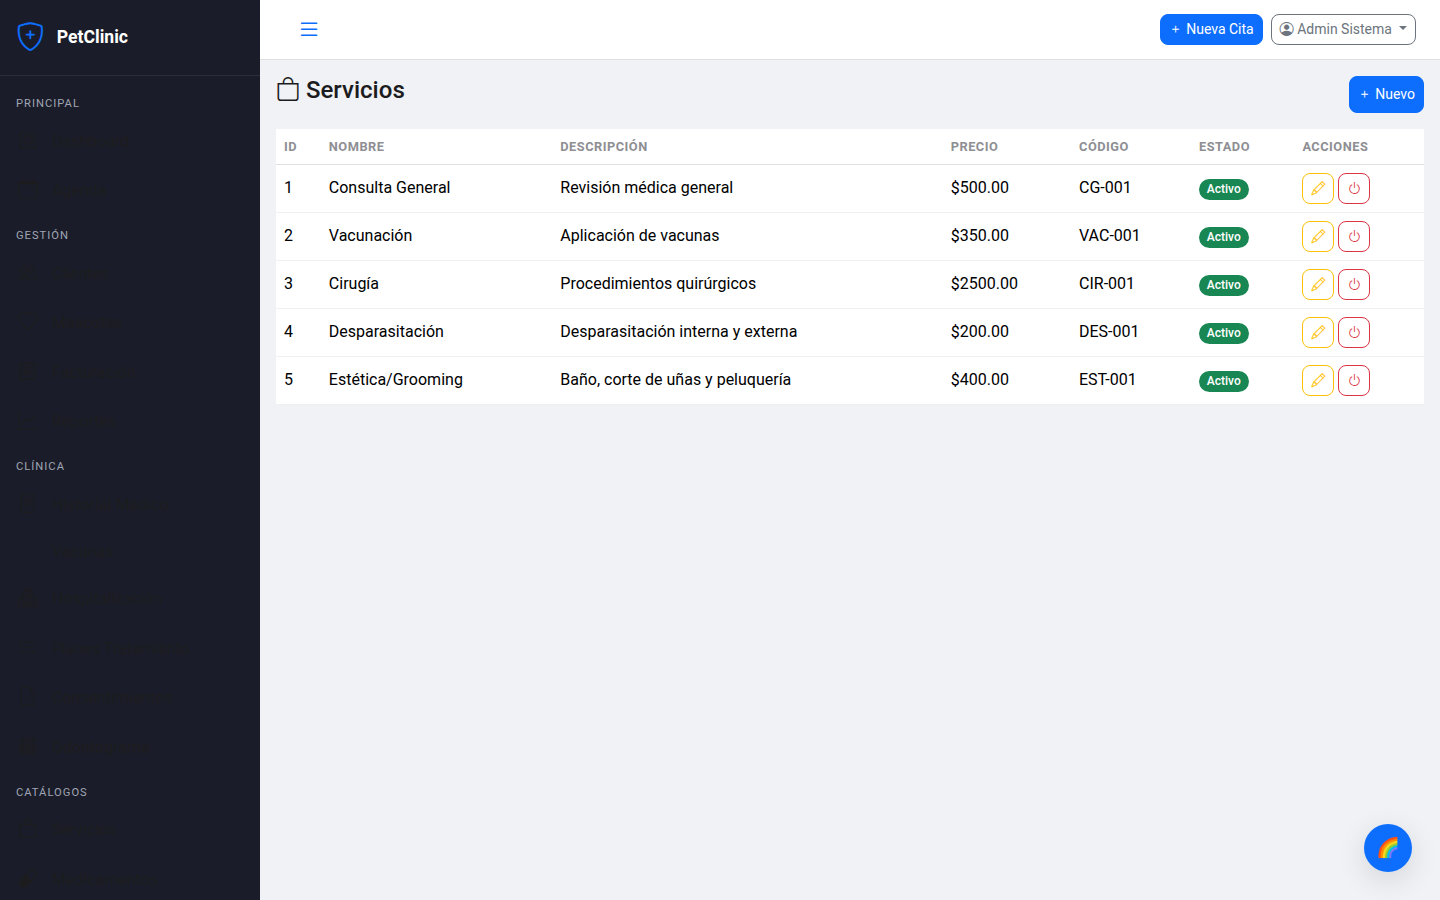
\includegraphics[width=0.9\textwidth]{images/14-servicios}
    \caption{Cat\'alogo de servicios con precios y activaci\'on}
    \label{fig:servicios}
\end{figure}

\section{M\'odulo de Medicamentos e Inventario}

Control de stock con trazabilidad completa de movimientos:

\begin{itemize}
    \item CRUD de medicamentos con unidad de medida y presentaci\'on.
    \item Control de stock m\'inimo con alertas visuales (stock bajo resaltado en rojo).
    \item Trazabilidad: cada movimiento registra tipo (entrada, salida, ajuste), cantidad, fecha y usuario.
    \item Descuento autom\'atico al facturar medicamentos.
    \item Vista de stock bajo (medicamentos con stock menor o igual al m\'inimo configurado).
\end{itemize}

\begin{figure}[H]
    \centering
    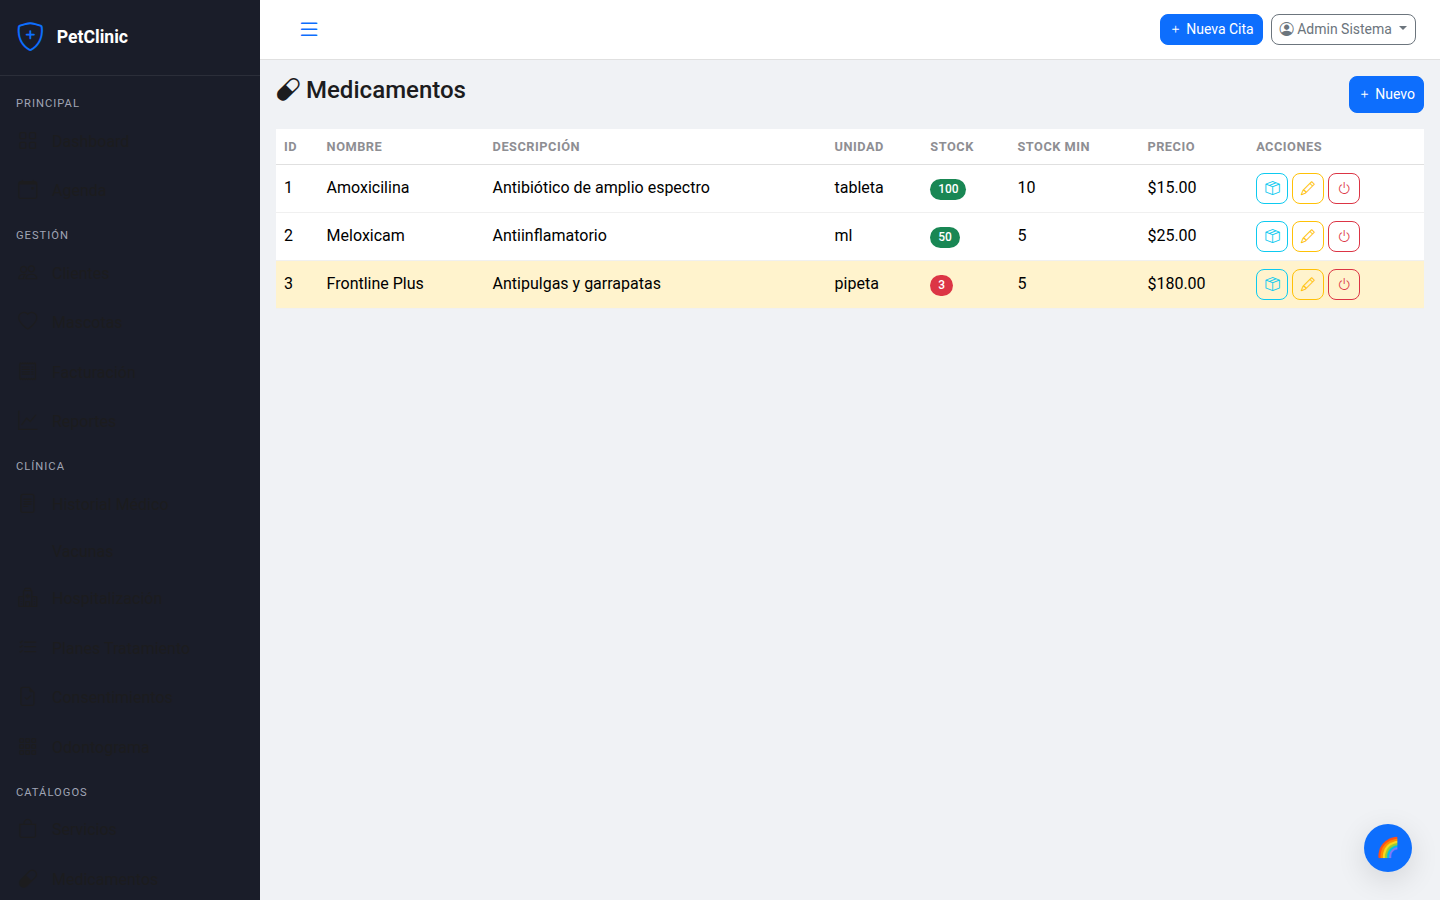
\includegraphics[width=0.9\textwidth]{images/15-medicamentos}
    \caption{Inventario de medicamentos con control de stock}
    \label{fig:medicamentos}
\end{figure}

\section{M\'odulo de Historial M\'edico}

Notas detalladas de consulta por mascota con orden cronol\'ogico:

\begin{itemize}
    \item Registro de motivo, diagn\'ostico, procedimiento y medicaci\'on recetada.
    \item Vinculaci\'on a citas espec\'ificas para contexto completo.
    \item Historial cronol\'ogico completo por mascota con b\'usqueda por fecha.
\end{itemize}

\begin{figure}[H]
    \centering
    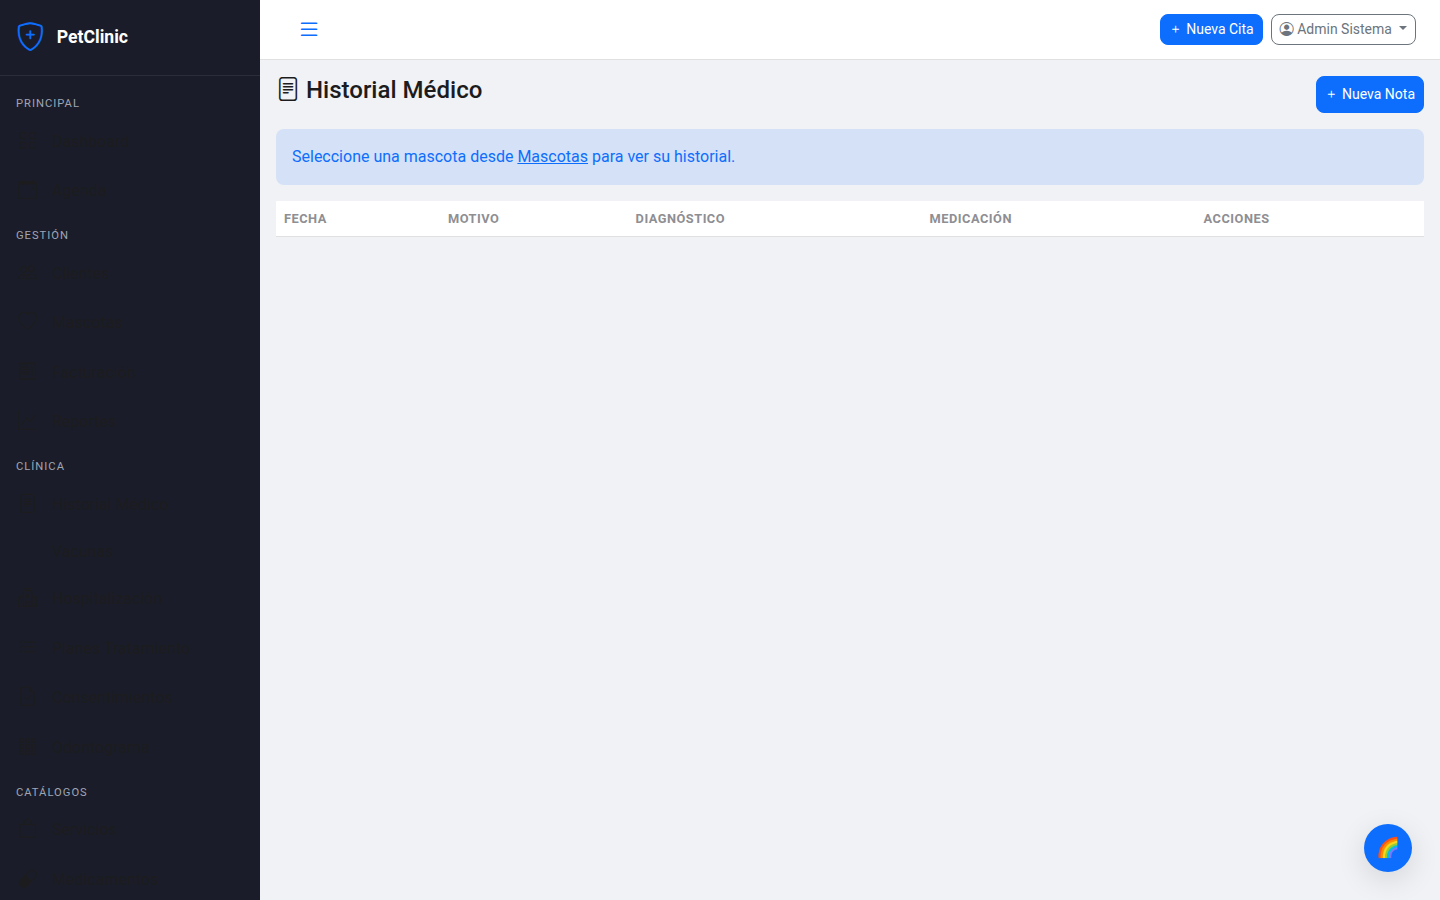
\includegraphics[width=0.9\textwidth]{images/08-historial-medico}
    \caption{Historial m\'edico de mascota con notas de consulta}
    \label{fig:historial}
\end{figure}

\section{M\'odulo de Vacunas}

Control de vacunaci\'on con alertas autom\'aticas por email:

\begin{itemize}
    \item Registro con nombre de vacuna, fecha de aplicaci\'on y pr\'oxima dosis.
    \item Control de lote y fabricante para trazabilidad.
    \item Alertas autom\'aticas por email: vacunas pr\'oximas a vencer (08:00) y vencidas (09:00).
    \item Tareas programadas con \texttt{@Scheduled} y cron expressions.
    \item Integraci\'on con JavaMailSender para env\'io de correos HTML con plantillas.
\end{itemize}

\begin{figure}[H]
    \centering
    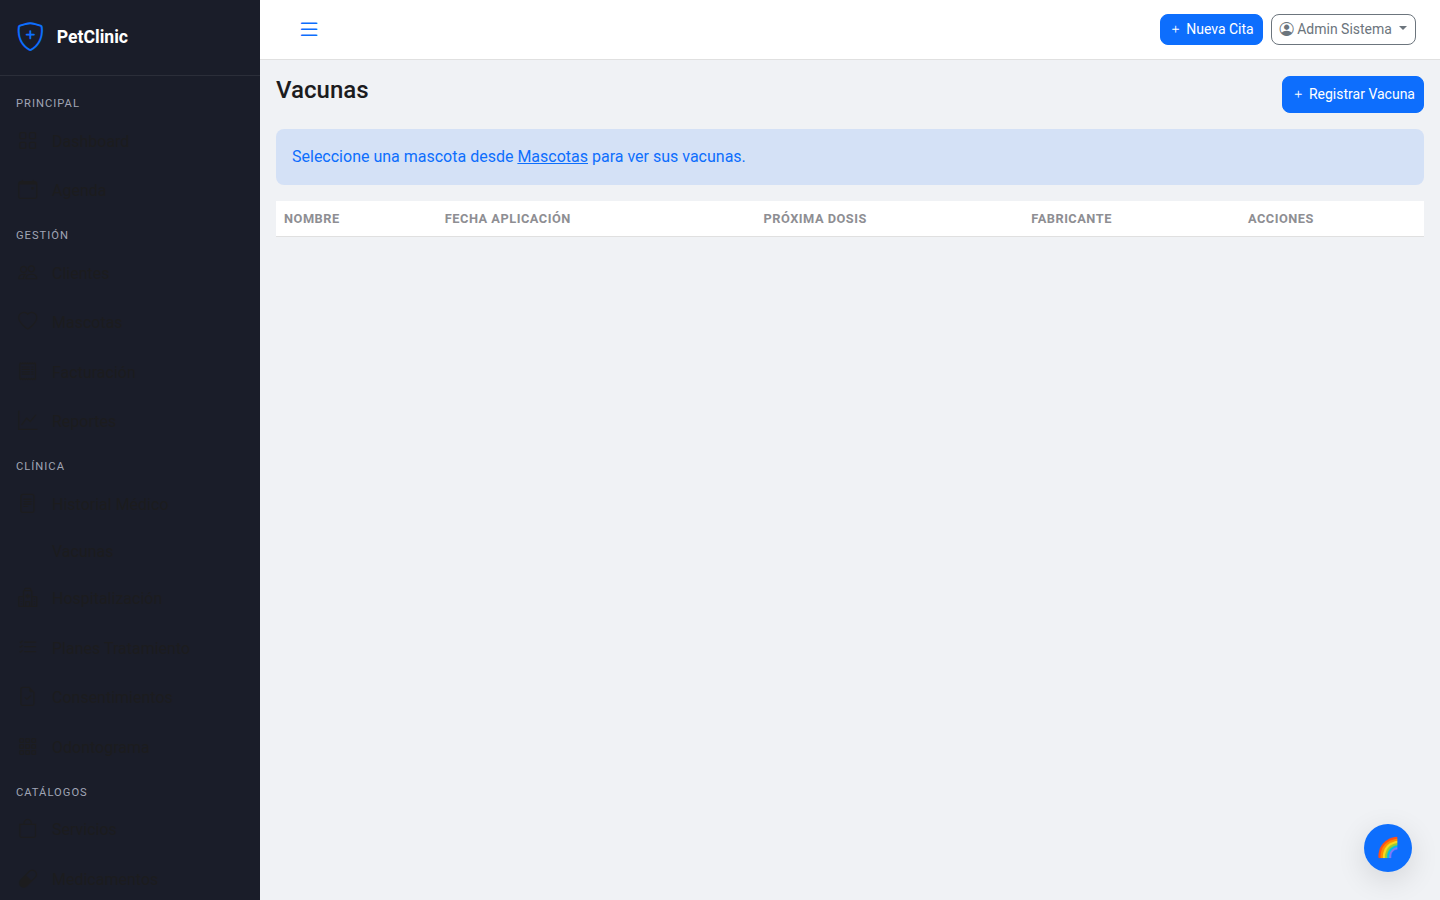
\includegraphics[width=0.9\textwidth]{images/09-vacunas}
    \caption{Registro de vacunas por mascota con alertas}
    \label{fig:vacunas}
\end{figure}

\section{M\'odulo de Hospitalizaci\'on}

Gesti\'on de pacientes hospitalizados con control de ingresos y altas:

\begin{itemize}
    \item Ingreso con asignaci\'on de jaula y motivo de hospitalizaci\'on.
    \item Control de check-in / check-out con fecha y hora exacta.
    \item Estado: Hospitalizado $\rightarrow$ Dado de Alta.
    \item Notas de evoluci\'on durante la estancia.
\end{itemize}

\begin{figure}[H]
    \centering
    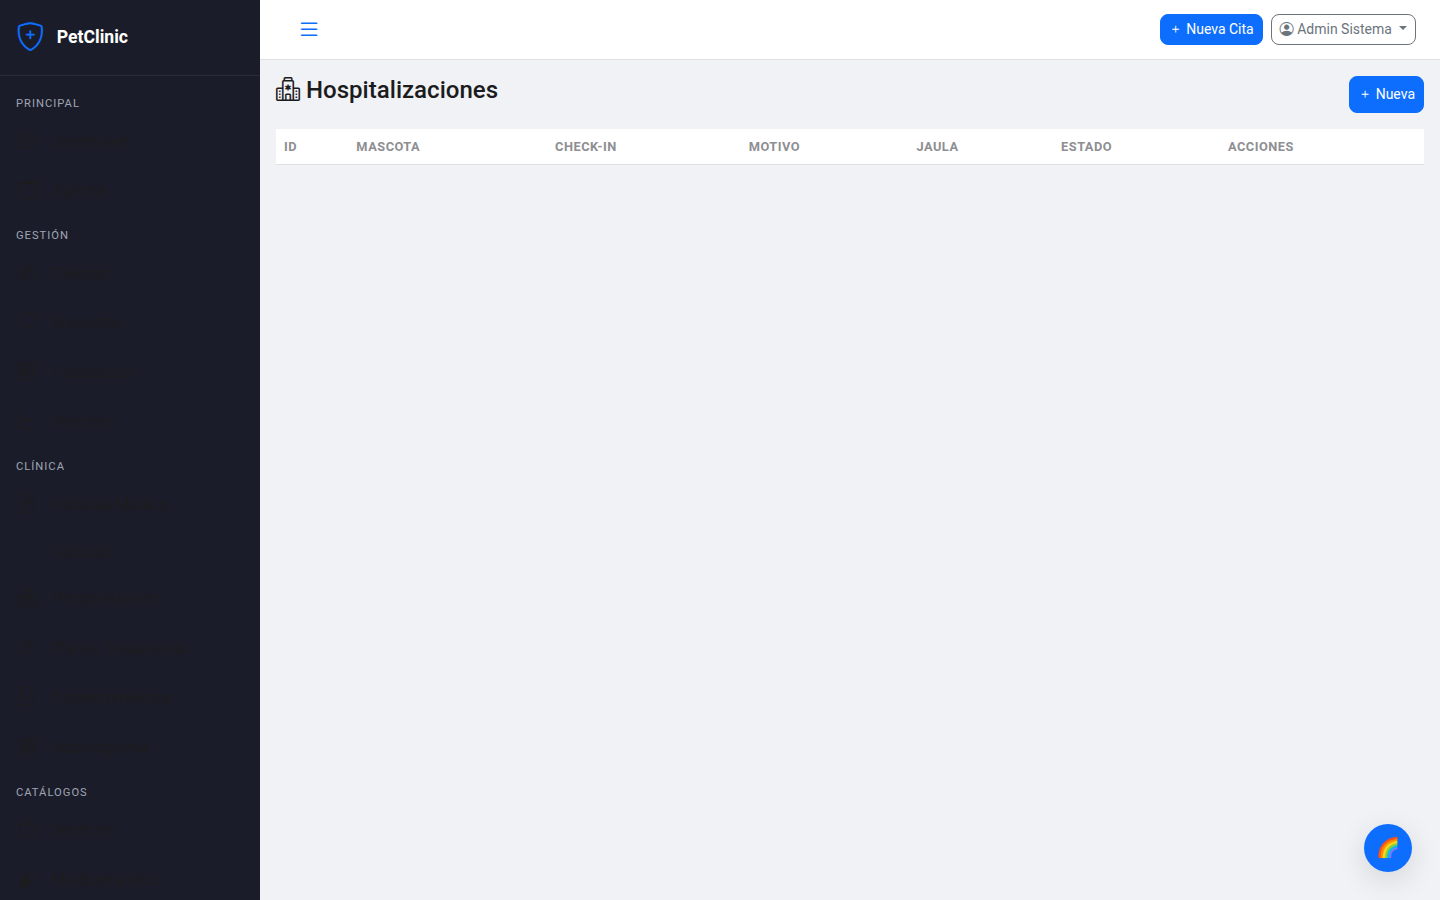
\includegraphics[width=0.9\textwidth]{images/10-hospitalizaciones}
    \caption{Pacientes hospitalizados con control de ingresos}
    \label{fig:hospitalizacion}
\end{figure}

\section{M\'odulo de Planes de Tratamiento}

Planes con pasos secuenciados para seguimiento de tratamientos:

\begin{itemize}
    \item Planes con t\'itulo, descripci\'on y costo estimado total.
    \item Pasos secuenciados con orden, servicio asociado y costo individual.
    \item Seguimiento de avance por paso: Pendiente $\rightarrow$ En Proceso $\rightarrow$ Completado $\rightarrow$ Omitido.
    \item Estados del plan: Activo, Completado, Cancelado.
\end{itemize}

\begin{figure}[H]
    \centering
    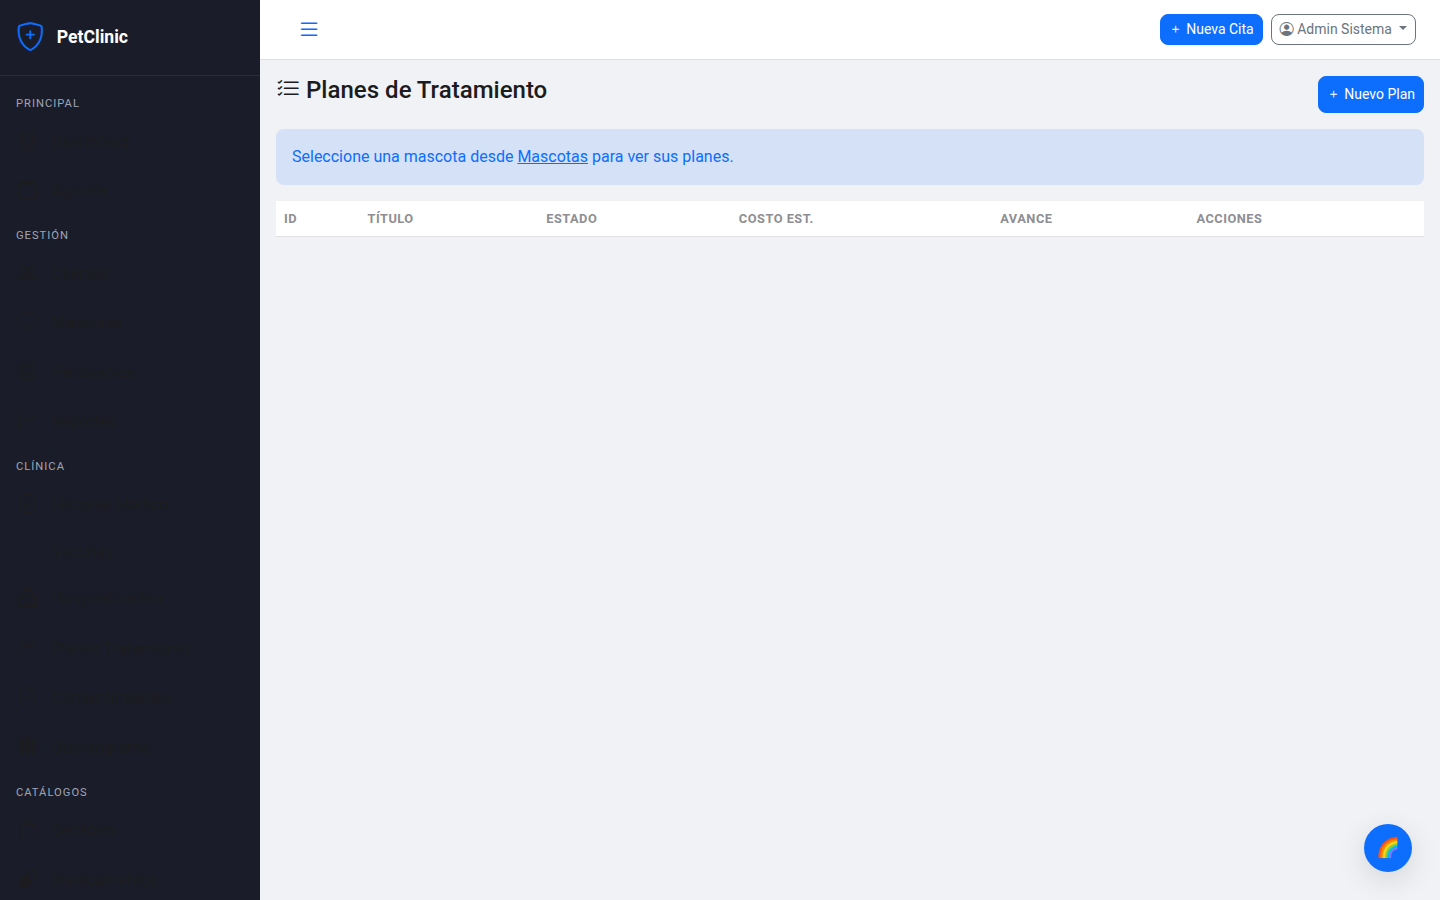
\includegraphics[width=0.9\textwidth]{images/11-planes-tratamiento}
    \caption{Plan de tratamiento con pasos secuenciados y avance}
    \label{fig:planes}
\end{figure}

\section{M\'odulo de Consentimientos Informados}

Documentos legales para procedimientos veterinarios:

\begin{itemize}
    \item Creaci\'on de documentos con t\'itulo, tipo de procedimiento y contenido detallado.
    \item Firma digital con registro de fecha, nombre completo del firmante y relaci\'on con la mascota.
    \item Generaci\'on de PDF profesional para impresi\'on y respaldo.
    \item Control de estado: Pendiente de Firma / Firmado.
\end{itemize}

\begin{figure}[H]
    \centering
    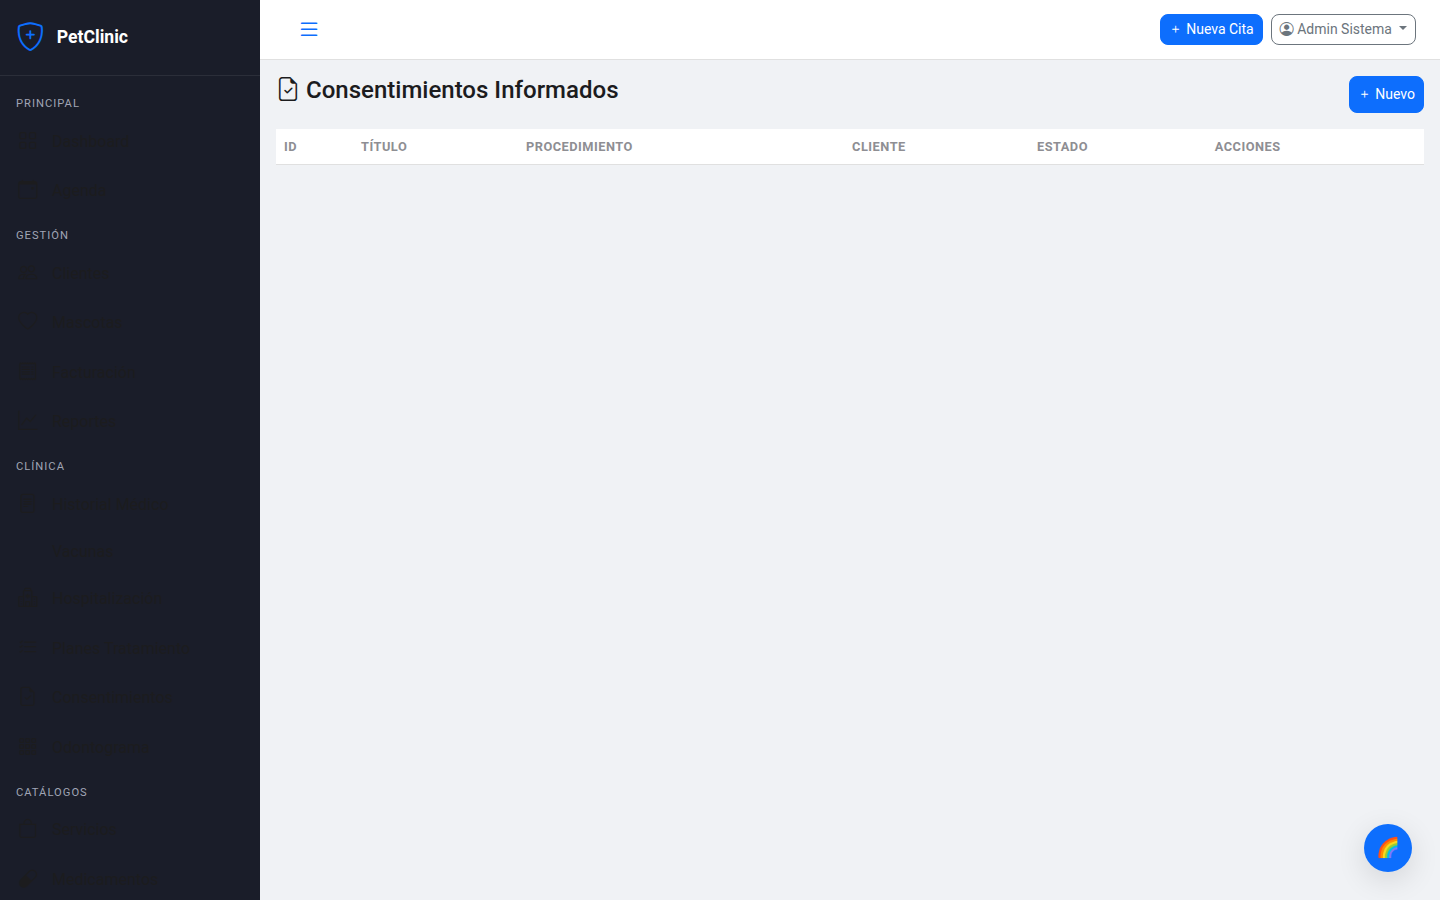
\includegraphics[width=0.9\textwidth]{images/12-consentimientos}
    \caption{Consentimiento informado con firma digital y PDF}
    \label{fig:consentimientos}
\end{figure}

\section{M\'odulo de Odontograma}

Diagrama dental canino interactivo implementado con HTML Canvas:

\begin{itemize}
    \item 42 dientes numerados seg\'un f\'ormula dental canina (I 3/3, C 1/1, P 4/4, M 2/3).
    \item Estados: SANO, T\'ARTARO, CARIES, FRACTURA, AUSENTE, PERIODONTAL, OBTURADO, ENDODONCIA.
    \item Cada estado se representa con un color diferente para identificaci\'on visual r\'apida.
    \item Interfaz interactiva: seleccionar estado en la leyenda y hacer clic en el diente.
    \item Persistencia de m\'ultiples odontogramas por mascota (uno por consulta dental).
\end{itemize}

\section{M\'odulo de Pagos Online (Stripe)}

Integraci\'on con Stripe Payment Intents para pagos en l\'inea:

\begin{itemize}
    \item Creaci\'on de intenci\'on de pago vinculada a una factura espec\'ifica.
    \item Modal simulado cuando Stripe no est\'a configurado (\textit{sandbox mode}).
    \item Webhook \texttt{/api/pagos/stripe/webhook} para confirmaci\'on as\'incrona de pagos.
    \item Actualizaci\'on autom\'atica del estado de la factura al confirmar el pago.
\end{itemize}

\section{M\'odulo de Reserva P\'ublica}

Permite a clientes potenciales agendar citas sin autenticaci\'on:

\begin{itemize}
    \item Listado de veterinarios disponibles con horarios y especialidades.
    \item Visualizaci\'on de slots disponibles por fecha y veterinario.
    \item Validaci\'on de email del cliente contra la base de datos existente.
    \item Creaci\'on de cita como visitante sin necesidad de registro.
\end{itemize}

\section{M\'odulo de Reportes}

An\'alisis de ingresos con visualizaci\'on gr\'afica y exportaci\'on:

\begin{itemize}
    \item Dashboard con 7 indicadores clave del sistema.
    \item Reporte de ingresos por per\'iodo con gr\'afico de barras (Chart.js).
    \item Exportaci\'on a Excel con Apache POI para an\'alisis externo.
    \item Filtro por rango de fechas personalizado.
\end{itemize}

\section{M\'odulo de Auditor\'ia}

Registro de todas las acciones importantes del sistema para cumplimiento y trazabilidad:

\begin{itemize}
    \item Log de acciones CREATE, UPDATE, DELETE con tipo de operaci\'on.
    \item Detalle de entidad afectada y usuario responsable.
    \item Registro de direcci\'on IP del cliente.
    \item Visualizaci\'on en tabla cronol\'ogica con filtros por entidad y fecha.
\end{itemize}

\begin{figure}[H]
    \centering
    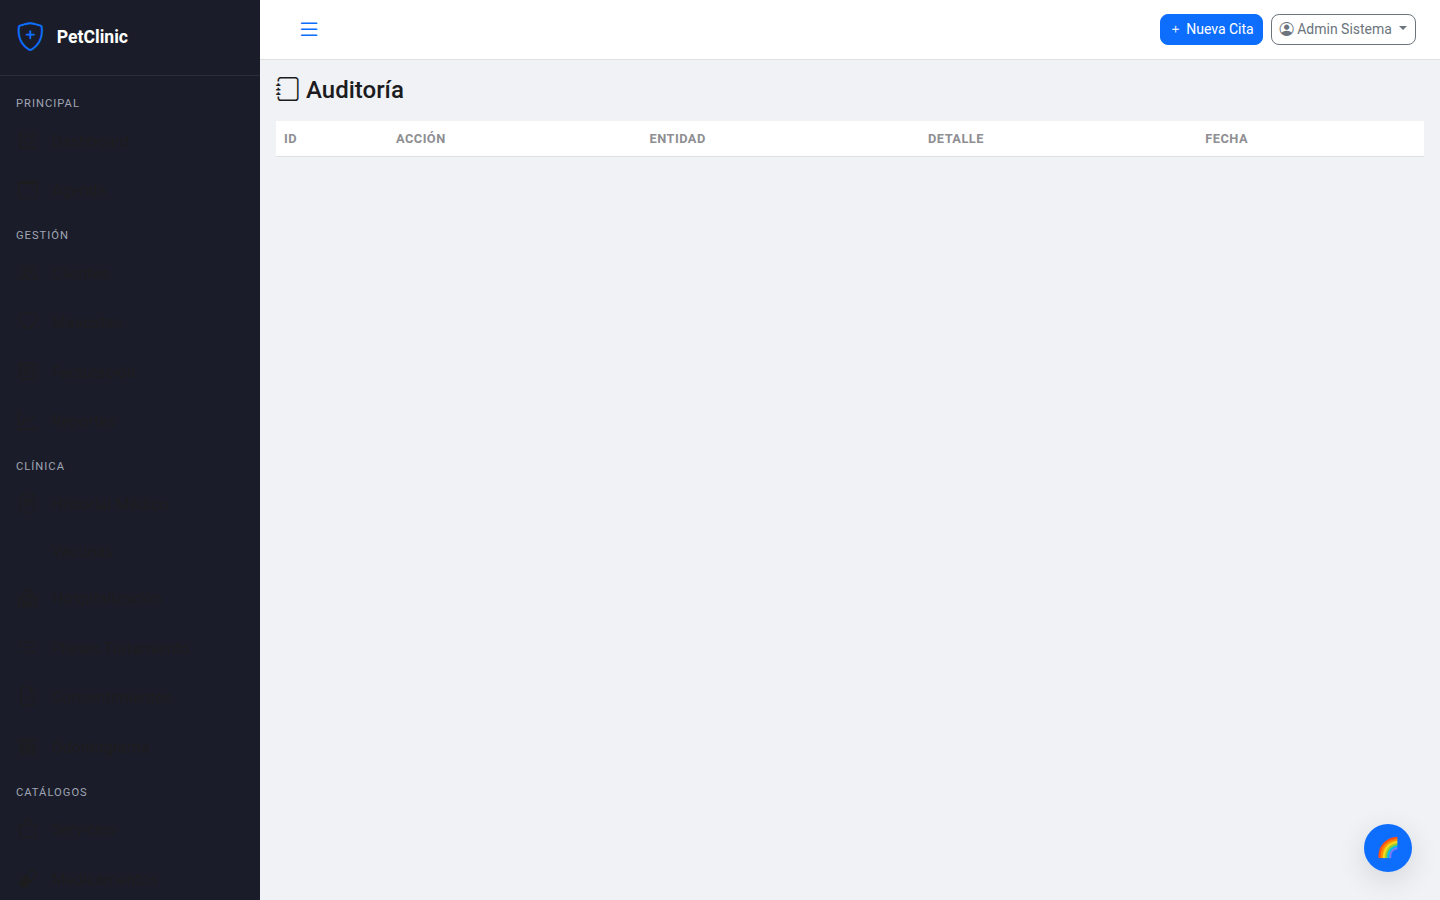
\includegraphics[width=0.9\textwidth]{images/17-auditoria}
    \caption{Log de auditor\'ia con acciones del sistema}
    \label{fig:auditoria2}
\end{figure}

\section{M\'odulo de Configuraci\'on}

Panel de configuraci\'on general del sistema:

\begin{itemize}
    \item Configuraci\'on de datos de la cl\'inica (nombre, direcci\'on, tel\'efono, email).
    \item Configuraci\'on de par\'ametros de facturaci\'on (impuestos, formato de n\'umero).
    \item Configuraci\'on de notificaciones (activar/desactivar alertas por email).
\end{itemize}

\begin{figure}[H]
    \centering
    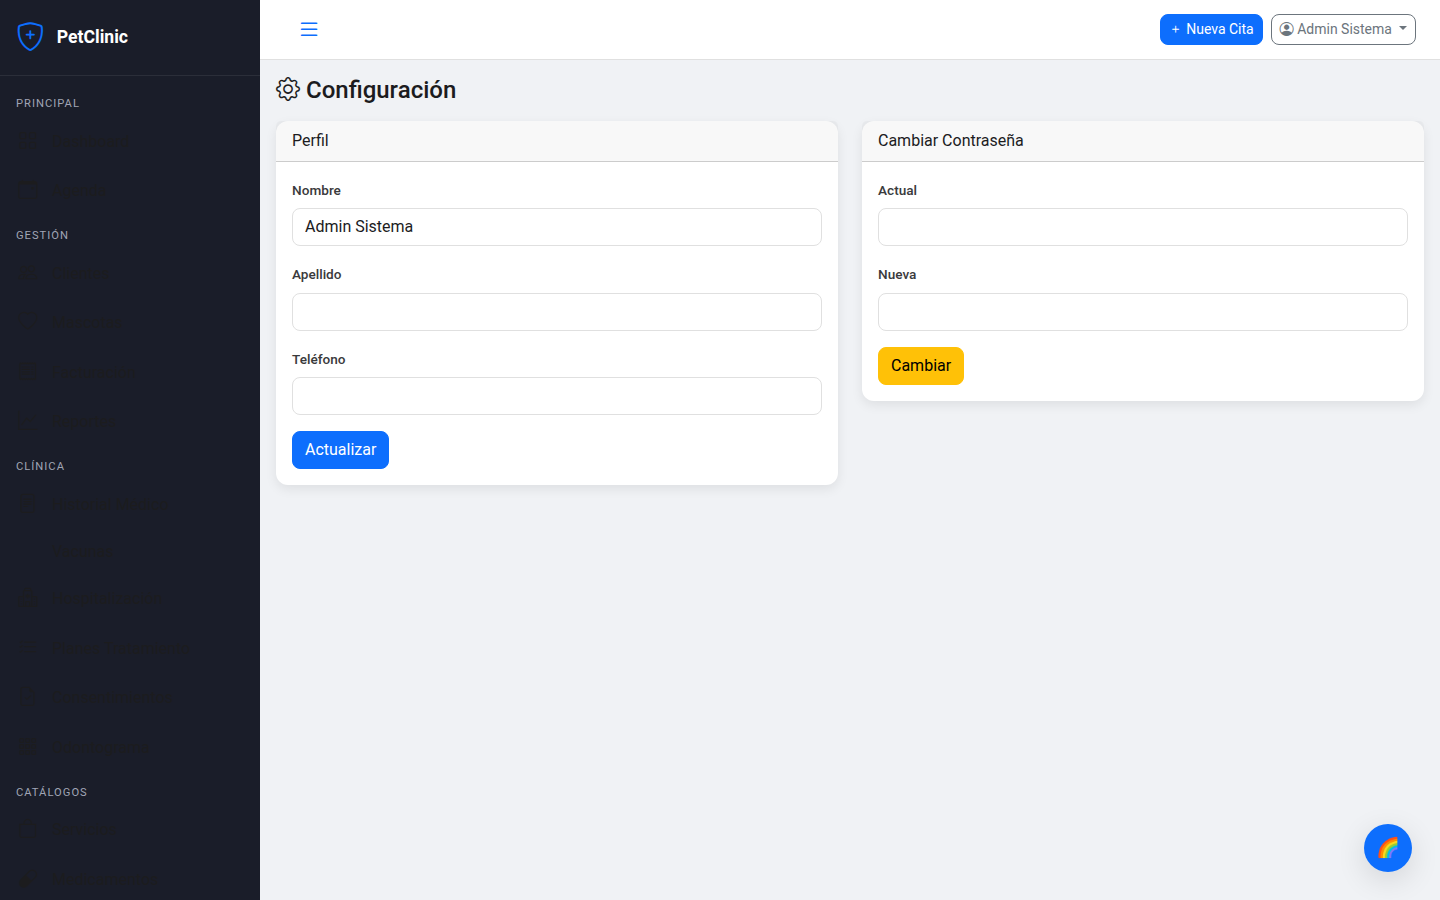
\includegraphics[width=0.9\textwidth]{images/18-configuracion}
    \caption{Panel de configuraci\'on general del sistema}
    \label{fig:config}
\end{figure}

\section{M\'odulo de Notificaciones}

Sistema de alertas multicanal con tareas programadas:

\begin{itemize}
    \item Alertas de vacunaci\'on por email (vacunas pr\'oximas a vencer y vencidas).
    \item Notificaciones autom\'aticas diarias v\'ia \texttt{@Scheduled} a las 08:00 y 09:00.
    \item Recordatorios de citas por email al momento de creaci\'on.
    \item Notificaciones de facturaci\'on (factura creada, pago recibido).
    \item Integraci\'on con JavaMailSender (SMTP) y plantillas HTML personalizables.
\end{itemize}

\begin{lstlisting}[language=Java, caption=Programaci\'on de alertas de vacunaci\'on]
@Component
public class VacunaScheduler {

    @Scheduled(cron = "0 0 8 * * ?")  // 08:00 todos los dias
    public void alertarProximasVacunas() {
        LocalDate hoy = LocalDate.now();
        LocalDate enDosSemanas = hoy.plusDays(14);
        List<Vacuna> proximas = vacunaRepo
            .findByFechaProximaDosisBetween(hoy, enDosSemanas);
        for (Vacuna v : proximas) {
            notificacionService.enviarAlertaVacunacion(v);
        }
    }

    @Scheduled(cron = "0 0 9 * * ?")  // 09:00 todos los dias
    public void alertarVacunasVencidas() {
        List<Vacuna> vencidas = vacunaRepo
            .findByFechaProximaDosisBefore(LocalDate.now());
        for (Vacuna v : vencidas) {
            notificacionService.enviarAlertaVacunacion(v);
        }
    }
}
\end{lstlisting}

\section{Sistema de Temas}

Personalizaci\'on visual con 8 temas de color intercambiables en tiempo real:

\begin{itemize}
    \item Implementado mediante variables CSS (\textit{Custom Properties}) en el elemento \texttt{:root}.
    \item Persistencia en \texttt{localStorage} para recordar el tema entre sesiones.
    \item Aplicaci\'on en tiempo real sin recarga de p\'agina.
    \item Bot\'on flotante en esquina inferior derecha con selector de temas.
    \item Integraci\'on con FullCalendar (actualiza colores del calendario al cambiar tema).
\end{itemize}

\section{Credenciales de Prueba}

\begin{longtable}{|p{3cm}|p{4cm}|p{3cm}|p{4cm}|}
\hline
\textbf{Rol} & \textbf{Email} & \textbf{Password} & \textbf{Descripci\'on} \\
\hline
ADMIN & admin@petclinic.com & Admin123 & Acceso total al sistema \\
VETERINARIO & vet@petclinic.com & Vet123 & Gesti\'on cl\'inica completa \\
RECEPCIONISTA & recepcion@petclinic.com & Recep123 & Lectura y creaci\'on b\'asica \\
CLIENTE & ana@email.com & Ana123 & Portal del cliente \\
\hline
\end{longtable}

\chapter{Pruebas}

\section{Enfoque de Pruebas}

El proyecto utiliza pruebas de integraci\'on con JUnit 5 y Spring Boot Test. Las pruebas se ejecutan contra una base de datos H2 en memoria, lo que permite validar el funcionamiento completo del sistema sin dependencias externas. Se siguen las siguientes pr\'acticas:

\begin{itemize}
    \item \textbf{Orden de ejecuci\'on:} Las pruebas se ejecutan en orden (\texttt{@TestMethodOrder(MethodName)} o \texttt{@Order}) para mantener consistencia en el estado de la base de datos.
    \item \textbf{Autenticaci\'on previa:} Cada clase de prueba autentica primero al usuario correspondiente (admin, vet, cliente) y reutiliza el token JWT obtenido.
    \item \textbf{Data inicial:} Los datos de prueba se cargan mediante \texttt{DataInitializer} al iniciar el contexto de Spring.
    \item \textbf{Configuraci\'on aislada:} Archivo \texttt{application.properties} espec\'ifico para pruebas con H2 y logging reducido.
\end{itemize}

\section{Ejecuci\'on de Pruebas}

\begin{lstlisting}[caption=Comando para ejecutar todas las pruebas]
mvn test
\end{lstlisting}

Para ejecutar una prueba espec\'ifica:

\begin{lstlisting}[caption=Ejecutar prueba individual]
mvn test -Dtest=VeterinarySystemIntegrationTest
mvn test -Dtest=NewFeaturesIntegrationTest#testCreateFactura
\end{lstlisting}

\section{Clases de Prueba}

\subsection{VeterinarySystemIntegrationTest}

Contiene 15 pruebas de integraci\'on que cubren el flujo b\'asico del sistema:

\begin{enumerate}
    \item \texttt{testLoginAdmin}: Inicio de sesi\'on como administrador, obtenci\'on de JWT y verificaci\'on de claims.
    \item \texttt{testLoginVet}: Inicio de sesi\'on como veterinario con rol VETERINARIO.
    \item \texttt{testDashboard}: Acceso al dashboard con token de administrador.
    \item \texttt{testGetClientes}: Listado paginado de clientes.
    \item \texttt{testGetMascotas}: Listado de mascotas filtradas por cliente.
    \item \texttt{testCreateCita}: Creaci\'on de cita con validaci\'on de disponibilidad.
    \item \texttt{testGetServicios}: Consulta de servicios activos.
    \item \texttt{testGetMedicamentos}: Consulta de medicamentos activos.
    \item \texttt{testCreateFactura}: Creaci\'on de factura con descuento autom\'atico de stock.
    \item \texttt{testGetFacturaPdf}: Generaci\'on y verificaci\'on de PDF de factura.
    \item \texttt{testHistorialMedico}: Consulta de historial m\'edico por mascota.
    \item \texttt{testHospitalizaciones}: Listado de hospitalizaciones activas.
    \item \texttt{testPortalAccessDenied}: Verificaci\'on de que un veterinario no accede al portal de cliente.
    \item \texttt{testLoginCliente}: Inicio de sesi\'on como cliente y acceso al portal.
    \item \texttt{testDeleteCita}: Eliminaci\'on l\'ogica de cita.
\end{enumerate}

\begin{lstlisting}[language=Java, caption=Ejemplo: autenticaci\'on como admin y prueba de dashboard]
@SpringBootTest(webEnvironment = WebEnvironment.RANDOM_PORT)
@TestMethodOrder(MethodName.class)
class VeterinarySystemIntegrationTest {

    @Autowired private TestRestTemplate restTemplate;
    private static String adminToken;
    private static Long clienteId;
    private static Long facturaId;

    @Test
    @Order(1)
    void testLoginAdmin() {
        LoginRequest req = new LoginRequest("admin@petclinic.com",
            "Admin123", "PERSONAL");
        ResponseEntity<LoginResponse> res = restTemplate.postForEntity(
            "/api/auth/login", req, LoginResponse.class);
        assertEquals(HttpStatus.OK, res.getStatusCode());
        assertNotNull(res.getBody().getToken());
        adminToken = res.getBody().getToken();
    }

    @Test
    @Order(2)
    void testDashboard() {
        HttpHeaders headers = new HttpHeaders();
        headers.setBearerAuth(adminToken);
        HttpEntity<Void> entity = new HttpEntity<>(headers);

        ResponseEntity<Map> res = restTemplate.exchange(
            "/api/medico/dashboard", HttpMethod.GET, entity, Map.class);
        assertEquals(HttpStatus.OK, res.getStatusCode());
        assertNotNull(res.getBody().get("totalClientes"));
    }
}
\end{lstlisting}

\subsection{NewFeaturesIntegrationTest}

Contiene 15 pruebas adicionales que cubren funcionalidades nuevas y endpoints p\'ublicos:

\begin{enumerate}
    \item \texttt{testLoginAdmin / testLoginVet}: Pruebas de autenticaci\'on para ambos roles.
    \item \texttt{testPublicListVeterinarios}: Listado p\'ublico de veterinarios activos sin autenticaci\'on.
    \item \texttt{testPublicSlots}: Visualizaci\'on de slots disponibles para una fecha y veterinario.
    \item \texttt{testPublicSlotsInvalidVet}: Veterinario inv\'alido retorna 404.
    \item \texttt{testPublicCreateCita}: Creaci\'on de cita p\'ublica como visitante.
    \item \texttt{testPublicCreateCitaWrongEmail}: Email incorrecto retorna 400.
    \item \texttt{testCreateFacturaForPayment}: Creaci\'on de factura para prueba de pago.
    \item \texttt{testCreatePaymentIntentUnauthenticated}: Pago requiere autenticaci\'on (retorna 401).
    \item \texttt{testCreatePaymentIntent}: Creaci\'on de intenci\'on de pago Stripe.
    \item \texttt{testCreatePaymentIntentInvalidFactura}: Factura inv\'alida retorna 400.
    \item \texttt{testVacunasForMascota}: Listado de vacunas por mascota.
    \item \texttt{testCitaCreateTriggersNotification}: Creaci\'on de cita dispara notificaci\'on programada.
    \item \texttt{testAllNewServiceBeansExist}: Verificaci\'on de que todos los beans de servicios se cargan correctamente.
    \item \texttt{testPublicEndpointsNoAuthRequired}: Endpoints p\'ublicos accesibles sin token.
    \item \texttt{testPaymentEndpointRequiresAuth}: Endpoint de pago protegido correctamente.
\end{enumerate}

\section{Configuraci\'on de Pruebas}

Las pruebas utilizan una configuraci\'on espec\'ifica en \texttt{src/test/resources/application.properties}:

\begin{lstlisting}[caption=Configuraci\'on para pruebas de integraci\'on]
# Base de datos en memoria H2
spring.datasource.url=jdbc:h2:mem:testdb;DB_CLOSE_DELAY=-1
spring.datasource.driver-class-name=org.h2.Driver
spring.jpa.hibernate.ddl-auto=create-drop

# JWT para pruebas (clave fija)
app.jwt.secret=TestSecretKeyForTestingPurposesOnly2024!!
app.jwt.expiration=3600000

# Email desactivado en pruebas
spring.mail.port=-1

# Logging reducido para pruebas
logging.level.com.veterinary=WARN
\end{lstlisting}

\section{Ejemplo: Prueba de Creaci\'on de Factura con Descuento de Stock}

\begin{lstlisting}[language=Java, caption=Prueba de integraci\'on para creaci\'on de factura]
@Test
@Order(9)
void testCreateFactura() {
    HttpHeaders headers = new HttpHeaders();
    headers.setBearerAuth(adminToken);
    headers.setContentType(MediaType.APPLICATION_JSON);

    String body = """
    {
        "clienteId": %d,
        "detalles": [
            {"tipoItem": "SERVICIO", "servicioId": 1,
             "descripcionLinea": "Consulta General",
             "cantidad": 1, "precioUnitario": 500},
            {"tipoItem": "MEDICAMENTO", "medicamentoId": 1,
             "descripcionLinea": "Amoxicilina",
             "cantidad": 2, "precioUnitario": 15}
        ]
    }
    """.formatted(clienteId);

    HttpEntity<String> entity = new HttpEntity<>(body, headers);
    ResponseEntity<Map> res = restTemplate.exchange(
        "/api/medico/facturas", HttpMethod.POST, entity, Map.class);

    assertEquals(HttpStatus.OK, res.getStatusCode());
    assertNotNull(res.getBody().get("numeroFactura"));
    assertEquals(530.0, (Double) res.getBody().get("total"), 0.01);
    facturaId = ((Number) res.getBody().get("id")).longValue();
}
\end{lstlisting}

\section{Ejemplo: Prueba de Endpoints P\'ublicos}

\begin{lstlisting}[language=Java, caption=Prueba de agenda p\'ublica sin autenticaci\'on]
@Test
void testPublicSlots() {
    ResponseEntity<String> res = restTemplate.getForEntity(
        "/api/public/slots?vetId=1&fecha="
        + LocalDate.now().plusDays(1).toString(),
        String.class);
    assertEquals(HttpStatus.OK, res.getStatusCode());
    assertTrue(res.getBody().contains("hora"));
    assertTrue(res.getBody().contains("disponible"));
}

@Test
void testPublicEndpointsNoAuthRequired() {
    ResponseEntity<String> res = restTemplate.getForEntity(
        "/api/public/veterinarios", String.class);
    assertEquals(HttpStatus.OK, res.getStatusCode());
}
\end{lstlisting}

\section{Cobertura de Pruebas}

Las 30 pruebas de integraci\'on cubren las siguientes \'areas del sistema:

\begin{itemize}
    \item \textbf{Autenticaci\'on (6):} Login como ADMIN, VETERINARIO, RECEPCIONISTA y CLIENTE; validaci\'on de credenciales incorrectas; protecci\'on de endpoints.
    \item \textbf{CRUD (8):} Creaci\'on, lectura, actualizaci\'on y eliminaci\'on de entidades principales (clientes, mascotas, citas, facturas).
    \item \textbf{Reglas de negocio (5):} Validaci\'on de disponibilidad de citas, descuento de stock en facturaci\'on, control de acceso por roles, validaci\'on de email en reserva p\'ublica.
    \item \textbf{Integraci\'on (4):} WebSocket, notificaciones por email, generaci\'on de PDF con iText, exportaci\'on Excel.
    \item \textbf{Pagos (3):} Creaci\'on de Payment Intent, webhook de Stripe, protecci\'on de endpoint de pago.
    \item \textbf{Reserva p\'ublica (3):} Listado de veterinarios, slots disponibles, creaci\'on de cita sin autenticaci\'on.
    \item \textbf{Existencia de beans (1):} Verificaci\'on de que todos los servicios se cargan en el contexto de Spring.
\end{itemize}

\chapter{Despliegue}

\section{Requisitos del Servidor}

\begin{itemize}
    \item Java 21 o superior (OpenJDK 21 LTS recomendado).
    \item PostgreSQL 14 o superior.
    \item Maven 3.8+ (para compilaci\'on desde c\'odigo fuente).
    \item Al menos 512 MB de RAM para la aplicaci\'on (1 GB recomendado).
    \item Conexi\'on SMTP saliente para notificaciones por email (opcional).
    \item Cuenta de Stripe con API keys para pagos en l\'inea (opcional).
\end{itemize}

\section{Configuraci\'on de Base de Datos}

\subsection{Crear Base de Datos PostgreSQL}

\begin{lstlisting}[caption=Creaci\'on de base de datos y usuario en PostgreSQL]
sudo -u postgres psql -c "CREATE DATABASE veterinary_db;"
sudo -u postgres psql -c "CREATE USER veterinary_user WITH PASSWORD 'veterinary_pass';"
sudo -u postgres psql -c "GRANT ALL PRIVILEGES ON DATABASE veterinary_db TO veterinary_user;"
\end{lstlisting}

\subsection{Verificar Conexi\'on}

\begin{lstlisting}[caption=Verificar que la base de datos es accesible]
psql -U veterinary_user -d veterinary_db -h localhost
\end{lstlisting}

\section{Ejecuci\'on en Desarrollo}

\begin{lstlisting}[caption=Ejecutar la aplicaci\'on en modo desarrollo]
mvn spring-boot:run
\end{lstlisting}

La aplicaci\'on estar\'a disponible en \texttt{http://localhost:8090}. La base de datos se crea y puebla autom\'aticamente al primer inicio gracias a \texttt{spring.jpa.hibernate.ddl-auto=update} y el \texttt{DataInitializer}.

\section{Compilaci\'on para Producci\'on}

\begin{lstlisting}[caption=Compilar y empaquetar como JAR]
mvn clean package -DskipTests
\end{lstlisting}

Genera el archivo \texttt{target/veterinary-clinic-management-system-1.0.0.jar}.

\begin{lstlisting}[caption=Ejecutar JAR compilado con variables de entorno]
export JWT_SECRET="clave-secreta-muy-segura-12345"
export JWT_EXPIRATION=1800000
export MAIL_HOST=smtp.gmail.com
export MAIL_USERNAME=notificaciones@petclinic.com
export MAIL_PASSWORD=contrasena-de-app
export STRIPE_API_KEY=sk_live_...
export STRIPE_WEBHOOK_SECRET=whsec_...

java -jar target/veterinary-clinic-management-system-1.0.0.jar
\end{lstlisting}

\section{Despliegue con Docker}

\subsection{Dockerfile}

\begin{lstlisting}[caption=Dockerfile multi-etapa para imagen optimizada]
FROM maven:3.9-eclipse-temurin-21 AS builder
WORKDIR /app
COPY pom.xml .
RUN mvn dependency:go-offline
COPY src ./src
RUN mvn clean package -DskipTests

FROM openjdk:21-jdk-slim
WORKDIR /app
COPY --from=builder /app/target/*.jar app.jar
EXPOSE 8090
ENTRYPOINT ["java", "-jar", "/app/app.jar"]
\end{lstlisting}

\subsection{Docker Compose}

\begin{lstlisting}[caption=Docker Compose con PostgreSQL y aplicaci\'on]
version: '3.8'
services:
  postgres:
    image: postgres:14
    environment:
      POSTGRES_DB: veterinary_db
      POSTGRES_USER: veterinary_user
      POSTGRES_PASSWORD: veterinary_pass
    ports:
      - "5432:5432"
    volumes:
      - postgres_data:/var/lib/postgresql/data

  app:
    build: .
    ports:
      - "8090:8090"
    environment:
      SPRING_DATASOURCE_URL: jdbc:postgresql://postgres:5432/veterinary_db
      SPRING_DATASOURCE_USERNAME: veterinary_user
      SPRING_DATASOURCE_PASSWORD: veterinary_pass
      JWT_SECRET: clave-secreta-docker-2024
      JWT_EXPIRATION: 1800000
    depends_on:
      - postgres

volumes:
  postgres_data:
\end{lstlisting}

\begin{lstlisting}[caption=Construir y ejecutar con Docker Compose]
docker-compose build
docker-compose up -d
docker-compose logs -f app  # Ver logs en tiempo real
\end{lstlisting}

\section{Despliegue con systemd (Producci\'on Linux)}

Para ejecutar la aplicaci\'on como servicio del sistema:

\begin{lstlisting}[caption=Archivo de servicio systemd]
[Unit]
Description=PetClinic Veterinary Clinic
After=network.target postgresql.service

[Service]
Type=simple
User=petclinic
WorkingDirectory=/opt/petclinic
Environment="JWT_SECRET=..."
Environment="JWT_EXPIRATION=1800000"
Environment="MAIL_HOST=smtp.gmail.com"
ExecStart=/usr/bin/java -jar /opt/petclinic/app.jar
Restart=on-failure
RestartSec=10

[Install]
WantedBy=multi-user.target
\end{lstlisting}

\begin{lstlisting}[caption=Instalar y gestionar el servicio]
sudo cp petclinic.service /etc/systemd/system/
sudo systemctl daemon-reload
sudo systemctl enable petclinic
sudo systemctl start petclinic
sudo systemctl status petclinic
\end{lstlisting}

\section{Proxy Inverso con Nginx}

Para entornos de producci\'on con dominio propio:

\begin{lstlisting}[caption=Configuraci\'on de Nginx como proxy inverso]
server {
    listen 80;
    server_name petclinic.midominio.com;

    location / {
        proxy_pass http://localhost:8090;
        proxy_set_header Host $host;
        proxy_set_header X-Real-IP $remote_addr;
        proxy_set_header X-Forwarded-For $proxy_add_x_forwarded_for;
        proxy_set_header X-Forwarded-Proto $scheme;
    }

    location /ws {
        proxy_pass http://localhost:8090;
        proxy_http_version 1.1;
        proxy_set_header Upgrade $http_upgrade;
        proxy_set_header Connection "upgrade";
        proxy_set_header Host $host;
    }
}
\end{lstlisting}

\section{Variables de Entorno}

El sistema soporta configuraci\'on mediante variables de entorno para entornos productivos, lo que permite despliegues sin modificar archivos de configuraci\'on:

\begin{longtable}{|p{4cm}|p{6cm}|p{4cm}|}
\hline
\textbf{Variable} & \textbf{Descripci\'on} & \textbf{Valor por Defecto} \\
\hline
JWT\_SECRET & Clave secreta para firmar tokens JWT (HMAC-SHA384) & (valor interno) \\
JWT\_EXPIRATION & Duraci\'on del token en milisegundos & 1800000 (30 min) \\
MAIL\_HOST & Servidor SMTP para env\'io de correos & smtp.gmail.com \\
MAIL\_PORT & Puerto SMTP & 587 \\
MAIL\_USERNAME & Usuario SMTP & (vac\'io) \\
MAIL\_PASSWORD & Contrase\~na SMTP & (vac\'io) \\
STRIPE\_API\_KEY & Clave API de Stripe (pk\_/sk\_) & sk\_test\_placeholder \\
STRIPE\_WEBHOOK\_SECRET & Secreto de webhook Stripe & whsec\_placeholder \\
FRONTEND\_URL & URL del frontend para enlaces en emails & http://localhost:8090 \\
UPLOAD\_DIR & Directorio de subida de archivos & ./uploads \\
\hline
\end{longtable}

\section{Estructura Completa del Proyecto}

\begin{verbatim}
veterinary-clinic-management-system/
  |-- pom.xml                          # Dependencias Maven
  |-- README.md                        # Instrucciones rapidas
  |-- .gitignore
  |-- Dockerfile                       # Imagen Docker multi-etapa
  |-- docker-compose.yml               # Orquestacion Docker
  |-- docs/                            # Documentacion LaTeX
  |   |-- main.tex
  |   |-- chapters/
  |   |-- images/
  |-- src/
      |-- main/
      |   |-- java/com/veterinary/
      |   |   |-- VeterinaryApplication.java
      |   |   |-- config/
      |   |   |-- controller/          # 20 REST controllers
      |   |   |-- domain/              # 20 entidades + 9 enums
      |   |   |-- dto/                 # 6 DTOs
      |   |   |-- repository/          # 19 repositorios
      |   |   |-- scheduler/
      |   |   |-- security/            # 4 clases de seguridad
      |   |   |-- service/             # 22 servicios
      |   |-- resources/
      |       |-- application.properties
      |       |-- static/
      |           |-- index.html
      |           |-- css/app.css
      |           |-- js/{api.js, app.js, vet-extras.js}
      |-- test/
          |-- java/com/veterinary/
          |   |-- VeterinarySystemIntegrationTest.java   # 15 tests
          |   |-- NewFeaturesIntegrationTest.java         # 15 tests
          |-- resources/
              |-- application.properties
\end{verbatim}

\section{Comandos \'Utiles}

\begin{longtable}{|p{6cm}|p{8cm}|}
\hline
\textbf{Comando} & \textbf{Descripci\'on} \\
\hline
mvn spring-boot:run & Ejecutar la aplicaci\'on en desarrollo \\
mvn clean install & Compilar y empaquetar \\
mvn test & Ejecutar pruebas unitarias y de integraci\'on \\
mvn test -Dtest=ClaseTest\#metodo & Ejecutar prueba espec\'ifica \\
docker-compose up -d & Desplegar con Docker Compose \\
docker-compose logs -f app & Ver logs de la aplicaci\'on \\
java -jar target/*.jar & Ejecutar JAR compilado \\
sudo systemctl start petclinic & Iniciar servicio systemd \\
\hline
\end{longtable}

\section{Resoluci\'on de Problemas}

\subsection{Error de Conexi\'on a Base de Datos}

Verificar que PostgreSQL est\'e en ejecuci\'on y accesible:

\begin{lstlisting}[caption=Verificar conexi\'on PostgreSQL]
sudo systemctl status postgresql
psql -U veterinary_user -d veterinary_db -h localhost
\end{lstlisting}

Si el error persiste, verificar que \texttt{pg\_hba.conf} permita conexiones locales con autenticaci\'on por contrase\~na.

\subsection{Puerto Ocupado}

Si el puerto 8090 ya est\'a en uso, se puede cambiar en \texttt{application.properties} o v\'ia variable de entorno:

\begin{lstlisting}
server.port=8091
# O via entorno:
export SERVER_PORT=8091
\end{lstlisting}

\subsection{Error de Compilaci\'on}

Asegurar que Java 21 est\'e configurado correctamente:

\begin{lstlisting}
java -version  # Debe mostrar 21.x
mvn -version   # Debe usar Java 21
\end{lstlisting}

\subsection{Error de JWT}

Si los tokens JWT no se validan correctamente, verificar que \texttt{JWT\_SECRET} tenga al menos 256 bits (32 caracteres) y sea consistente entre reinicios de la aplicaci\'on.

\subsection{WebSocket no conecta}

Verificar que el proxy inverso (si existe) tenga configurada la actualizaci\'on de protocolo WebSocket (\texttt{Upgrade} y \texttt{Connection} headers). Para Nginx, asegurar que la ubicaci\'on \texttt{/ws} tenga las directivas \texttt{proxy\_set\_header Upgrade} y \texttt{proxy\_set\_header Connection "upgrade"}.


\end{document}
